\documentclass[11pt,letterpaper]{article}

% ---------- Page geometry ----------
\usepackage[margin=1in]{geometry}

% ---------- Graphics and floats ----------
\usepackage{graphicx}
\usepackage{float}

% ---------- Tables ----------
\usepackage{booktabs}
\usepackage{tabularx}

% ---------- Captions ----------
\usepackage[font=small,labelfont=bf]{caption}

% ---------- Lists ----------
\usepackage{enumitem}
\setlist{itemsep=2pt, topsep=4pt}

% Paragraph spacing: blank line between paragraphs, but keep first-line indent
\setlength{\parskip}{0.6em}
\setlength{\parindent}{1.5em}

% ---------- Colors ----------
\usepackage{xcolor}
\definecolor{codegreen}{rgb}{0.0,0.5,0.0}
\definecolor{codegray}{rgb}{0.5,0.5,0.5}
\definecolor{codepurple}{rgb}{0.58,0.0,0.82}
\definecolor{backcolour}{rgb}{0.96,0.96,0.94}
\definecolor{inlinecode}{HTML}{0B4F8E}

% Color inline code so identifiers stand out from prose without being loud.
\let\oldtexttt\texttt
\renewcommand{\texttt}[1]{{\color{inlinecode}\oldtexttt{#1}}}

% ---------- Listings ----------
\usepackage{listings}
\lstdefinestyle{mystyle}{
    backgroundcolor=\color{backcolour},
    commentstyle=\color{codegreen},
    keywordstyle=\color{blue},
    numberstyle=\tiny\color{codegray},
    stringstyle=\color{codepurple},
    basicstyle=\ttfamily\footnotesize,
    breakatwhitespace=false,
    breaklines=true,
    captionpos=b,
    keepspaces=true,
    numbers=left,
    numbersep=5pt,
    showspaces=false,
    showstringspaces=false,
    showtabs=false,
    tabsize=2,
    frame=single
}
\lstset{style=mystyle}

% Section start control: each \section begins on a fresh page so sections don't split awkwardly across pages
\usepackage{etoolbox}
\usepackage{needspace}
\preto\section{\clearpage}
\preto\subsection{\needspace{6\baselineskip}}
\preto\subsubsection{\needspace{5\baselineskip}}
\newcommand{\boldheading}[1]{\needspace{6\baselineskip}\noindent\textbf{#1}}

% Discourage orphan and widow lines so paragraphs don't strand single lines at page boundaries
\widowpenalty=10000
\clubpenalty=10000

% Allow ragged bottoms instead of stretching content to fill page heights
\raggedbottom

% MySQL keyword highlighting for SQL listings
\lstdefinelanguage{MySQL}{
    morekeywords={
        SELECT, FROM, WHERE, INSERT, INTO, VALUES, UPDATE, SET, DELETE,
        CREATE, TABLE, DATABASE, SCHEMA, DROP, ALTER, ADD, COLUMN, MODIFY,
        PRIMARY, KEY, FOREIGN, REFERENCES, NOT, NULL, DEFAULT, AUTO_INCREMENT,
        UNIQUE, INDEX, CONSTRAINT, CHECK, ON, DELETE, CASCADE, RESTRICT,
        JOIN, INNER, LEFT, RIGHT, OUTER, FULL, CROSS, USING, AS,
        GROUP, BY, ORDER, ASC, DESC, HAVING, LIMIT, OFFSET, DISTINCT, UNION,
        AND, OR, NOT, IN, BETWEEN, LIKE, IS, EXISTS, ANY, ALL,
        INT, INTEGER, BIGINT, SMALLINT, TINYINT, DECIMAL, NUMERIC, FLOAT, DOUBLE,
        CHAR, VARCHAR, TEXT, BLOB, DATE, DATETIME, TIMESTAMP, TIME, YEAR, BOOLEAN,
        BEGIN, COMMIT, ROLLBACK, TRANSACTION, START, SAVEPOINT,
        IF, THEN, ELSE, ELSEIF, END, CASE, WHEN, WHILE, DO, FOR, LOOP,
        PROCEDURE, FUNCTION, TRIGGER, VIEW, RETURNS, RETURN, DECLARE,
        GRANT, REVOKE, USER, ROLE, PRIVILEGES, IDENTIFIED,
        TRUE, FALSE, COUNT, SUM, AVG, MIN, MAX, NOW, CURRENT_TIMESTAMP
    },
    sensitive=false,
    morecomment=[l]{--},
    morecomment=[s]{/*}{*/},
    morestring=[b]',
    morestring=[b]"
}

% Bash style listing for shell commands
\lstdefinelanguage{Bash}{
    morekeywords={
        cd, ls, mkdir, rm, cp, mv, cat, echo, export, source, sudo,
        npm, npx, node, git, docker, mysql, pdflatex, curl, wget, chmod
    },
    sensitive=true,
    morecomment=[l]{\#},
    morestring=[b]',
    morestring=[b]"
}

% ---------- Hyperref last ----------
\usepackage[colorlinks=true, linkcolor=blue, urlcolor=blue, citecolor=blue]{hyperref}

% Limit TOC depth to sections + subsections only (no sub-subsections) so it stays compact
\setcounter{tocdepth}{2}

% ---------- Title metadata ----------
\title{Urban Scout: Unified Mobile Tourist Assistant \\ Final Project Report}
\author{Group 61 \\ Sean Kim \\ Muhtasim Ishmam \\ Talha Hussain Mahr}
\date{Winter 2026}

\begin{document}

\begin{titlepage}
    \centering

    \vspace*{1.5cm}

    {\large University of Calgary\par}
    \vspace{0.3cm}
    {\large Department of Computer Science\par}

    \vspace{0.8cm}
    {\Large CPSC 471 \textendash\ Database Management Systems\par}

    \vspace{1.0cm}
    \rule{\linewidth}{0.5mm}

    \vspace{1.2cm}
    {\Huge\bfseries Urban Scout\par}

    \vspace{0.6cm}
    {\LARGE Unified Mobile Tourist Assistant\par}

    \vspace{0.8cm}
    {\Large Final Project Report\par}

    \vspace{1.2cm}
    \rule{\linewidth}{0.5mm}

    \vspace{1.5cm}
    {\Large\bfseries Group 61\par}

    \vspace{1.0cm}
    \begin{tabular}{c}
        \Large Sean Kim \\[0.4em]
        \Large Muhtasim Ishmam \\[0.4em]
        \Large Talha Hussain Mahr \\
    \end{tabular}

    \vfill

    {\large Winter 2026\par}

    \vspace{0.5cm}
\end{titlepage}

\newpage

\begin{abstract}
\large
Urban Scout is a mobile-friendly web application designed to reduce the fragmentation of travel information for tourists navigating unfamiliar cities. In many real-world situations, travelers must switch between multiple platforms to access transit schedules, restaurant information, landmarks, local events, and safety updates. This creates inefficiency, confusion, and unnecessary cognitive overload, especially for short-term visitors who need quick and reliable access to location-based information. Urban Scout addresses this problem by integrating these services into a single relational database-backed system.

\vspace{1em}
The project was implemented using a MySQL database, an Express/Node.js backend, and a React frontend with a mobile-first interface. The system supports multiple user roles, primarily tourists and administrators. Tourists can browse places by region, view transit-related information, read localized news and safety alerts, submit incident reports, and manage itineraries. Administrators can manage news content and verify reported incidents. The database design emphasizes relational connections between regions, places, transit services, news posts, alerts, users, and itineraries, allowing the application to present connected information that would normally be spread across different platforms.

\vspace{1em}
Overall, Urban Scout demonstrates how a well-designed relational database can support a unified user experience for tourism-related planning and awareness. By combining transportation, destination browsing, local updates, and trip planning into one system, the project reduces app fatigue and improves usability for travelers on the go.
\end{abstract}


\tableofcontents
\newpage

\section{Introduction}

Modern tourism often depends on multiple disconnected digital services. A traveler may need one application for maps, another for transit schedules, another for restaurant recommendations, and yet another source for local news or safety-related updates. As a result, users are forced to repeatedly switch contexts and manually combine information from several unrelated platforms. This fragmented experience is inconvenient, time-consuming, and especially difficult for tourists who are unfamiliar with the area they are visiting.

Urban Scout was designed to address this problem by providing a centralized system for tourism-related information. The project focuses on integrating key categories of data that are often used together in practice: places of interest, eateries, transit stations and schedules, localized news, safety alerts, incident reports, and itineraries. Rather than treating these pieces of information as separate resources, Urban Scout connects them through a relational database structure so that users can interact with them in a unified way.

The system created for this project is a mobile-friendly web application supported by a MySQL relational database, an Express/Node.js backend, and a React frontend. The primary end users are tourists, who can explore regions, browse places, check transit information, read local updates, report incidents, and organize their travel plans. A secondary user group consists of administrators, who are responsible for posting regional news and verifying incident reports. Through this design, Urban Scout demonstrates how database-driven integration can improve usability and reduce the burden of managing travel information across multiple disconnected applications.

\section{Project Design}

\subsection{Real-World Scenario}

Urban Scout was designed around a realistic tourism scenario in which short-term visitors need quick access to multiple types of local information while moving through a city. In practice, tourists often rely on several disconnected platforms to plan their day. A traveler may use one service to find landmarks, another to locate restaurants, another to check transit schedules, and another to search for local events, closures, or safety concerns. This separation of information creates unnecessary friction, especially for users who are unfamiliar with the city and need fast, location-aware decisions.

The project models a tourism support system for Seoul, with data organized into major regions such as Downtown Seoul, Gangnam, and Hongdae. These regions help structure the application and allow the system to connect transit, destinations, local updates, and user activity in a meaningful way. By placing all of this information in one relational database, Urban Scout reduces context switching and allows users to interact with related information through a single interface.

\subsection{User Groups}

The system was designed for two primary categories of users: regular users and administrators.

\boldheading{Regular Users}

Regular users represent tourists or visitors using the platform to explore the city and organize their travel plans. Their main goals are to find places of interest, understand how to move between locations, stay informed about local conditions, and build simple itineraries.

The system allows regular users to:
\begin{itemize}
    \item log in using a seeded email account
    \item browse regions and subscribe to regions of interest
    \item view places such as landmarks, eateries, and transit stations
    \item access transit-related information for selected stations
    \item read region-based news and safety alerts
    \item submit incident reports connected to a region
    \item create and manage itineraries
    \item view their own submitted reports
\end{itemize}

These functions were chosen because they reflect common tourist needs: discovering what exists in an area, deciding where to go, understanding how to get there, and staying aware of ongoing events or hazards.

\boldheading{Administrators}

Administrators represent trusted system managers who maintain local updates and review user-submitted reports. Their role supports the reliability and usefulness of the platform.

The system allows administrators to:
\begin{itemize}
    \item log in through the admin interface
    \item access protected admin pages
    \item review incident reports submitted by users
    \item verify or update the status of reports
    \item create and manage regional news posts
    \item contribute to the safety and information layer of the application
    \item add new places (landmarks, eateries, transit stations) to a region
    \item add and remove transit routes and link station-vehicle pairs as stops on a route
\end{itemize}

This user group was included because the project is not only a read-only guide. It also models a system where information can be maintained and moderated, making the application more realistic and dynamic.

\subsection{Core Design Goals}

Several design goals guided the structure of the project.

\boldheading{Unified Information Access}

The main goal was to combine multiple categories of travel-related data into one database-backed system. Instead of forcing users to mentally connect unrelated apps, the system was designed to connect places, regions, transit, safety information, and itineraries through explicit relationships in the schema.

\boldheading{Relational Integration}

A central goal of the database design was to ensure that the major entities were meaningfully linked. For example:
\begin{itemize}
    \item each place belongs to a region
    \item transit stations are represented as places
    \item nearby places can be connected to stations
    \item news posts are associated with regions
    \item safety alerts are attached to news posts
    \item incident reports are tied to both users and regions
    \item itinerary items reference specific places
\end{itemize}

This relational structure is one of the most important aspects of the project because it supports the ``unified assistant'' concept at the data level, not just in the user interface.

\boldheading{Mobile-Friendly Interaction}

Because tourists are likely to use the system while moving through a city, the interface was designed with a mobile-first approach. Navigation was kept simple, page content was organized into cards and lists, and the app was built to work well on smaller screens. This goal influenced both the frontend layout and the choice to keep user actions straightforward.

\boldheading{Role-Based Access}

The project also aimed to support different types of users without overcomplicating the experience. Regular users and administrators have different responsibilities, so the system includes role-based access to ensure that only administrators can perform moderation tasks such as managing news or verifying reports.

\subsection{Major Entities and Relationships}

The ER design centers around a set of entities that model the tourism scenario.

\boldheading{Region}

A \texttt{Region} represents a major area of the city. Regions organize places, news, and user subscriptions. They help group related information and allow region-based browsing and filtering.

\boldheading{Place}

A \texttt{Place} is a general entity used to represent locations relevant to the user. This entity is specialized into subtypes such as landmarks, eateries, and transit stations. This design avoids duplication while allowing each subtype to store its own attributes.

\boldheading{Landmark, Eatery, and TransitStation}

These entities specialize \texttt{Place}:
\begin{itemize}
    \item \texttt{Landmark} stores landmark-specific details such as type and hours
    \item \texttt{Eatery} stores dining-related details such as average cost
    \item \texttt{TransitStation} stores transit-specific details such as station code
\end{itemize}

This specialization structure was chosen to reflect the fact that these entities share common location data but also have distinct properties.

\boldheading{PublicTransit and TransitRoute}

\texttt{PublicTransit} represents specific transit services such as subway lines, buses, or trains. \texttt{TransitRoute} provides route-level information such as route names and service hours. The relationships among routes, stations, and transit services allow the application to display schedules and station-level service information.

\boldheading{NewsPost and SafetyAlert}

\texttt{NewsPost} stores regional updates and local information. \texttt{SafetyAlert} is modeled as a weak entity attached to a news post, allowing a single news item to contain one or more specific alerts. This is useful for representing situations where a larger event has multiple localized impacts.

\boldheading{IncidentReport}

An \texttt{IncidentReport} stores user-submitted safety or hazard information. Each report is linked to the user who submitted it and the region in which it occurred. This allows the system to collect user-generated information while still preserving geographic context.

\boldheading{Itinerary and ItineraryItem}

\texttt{Itinerary} stores a user's travel plan. \texttt{ItineraryItem} is a weak entity that represents individual scheduled items within an itinerary. Each itinerary item can reference a place, allowing users to connect planned activities to actual destinations in the database.

\subsection{Relationship Design}

Several relationships were included to capture how the different entities interact in practice.

\begin{itemize}
    \item A user can subscribe to one or more regions.
    \item A user can create one or more itineraries.
    \item An itinerary includes one or more itinerary items.
    \item An itinerary item references a place.
    \item A place belongs to a region.
    \item An admin is assigned to a region.
    \item An admin can verify incident reports.
    \item A news post is published for a region.
    \item A news post can contain safety alerts.
    \item A transit route serves a transit station.
    \item A place can be associated with a nearby transit station through a proximity relationship.
\end{itemize}

These relationships were intentionally chosen to support the features visible in the interface. They are not abstract additions, each one supports either browsing, filtering, reporting, route display, or planning.

\subsection{ER Diagram}

The ER diagram for Urban Scout reflects the complete conceptual design of the project. It includes strong entities, weak entities, specialization, and many-to-many relationships resolved through associative structures.

The most notable features of the ER design are:
\begin{itemize}[nosep]
    \item specialization from \texttt{Place} into \texttt{Landmark}, \texttt{Eatery}, and \texttt{TransitStation}
    \item weak entity treatment of \texttt{SafetyAlert}
    \item weak entity treatment of \texttt{ItineraryItem}
    \item associative relationships connecting users to regions, places to stations, and routes to stations and transit services
\end{itemize}
\nopagebreak[4]

\begin{figure}[H]
    \centering
    \IfFileExists{figures/eer.png}{%
        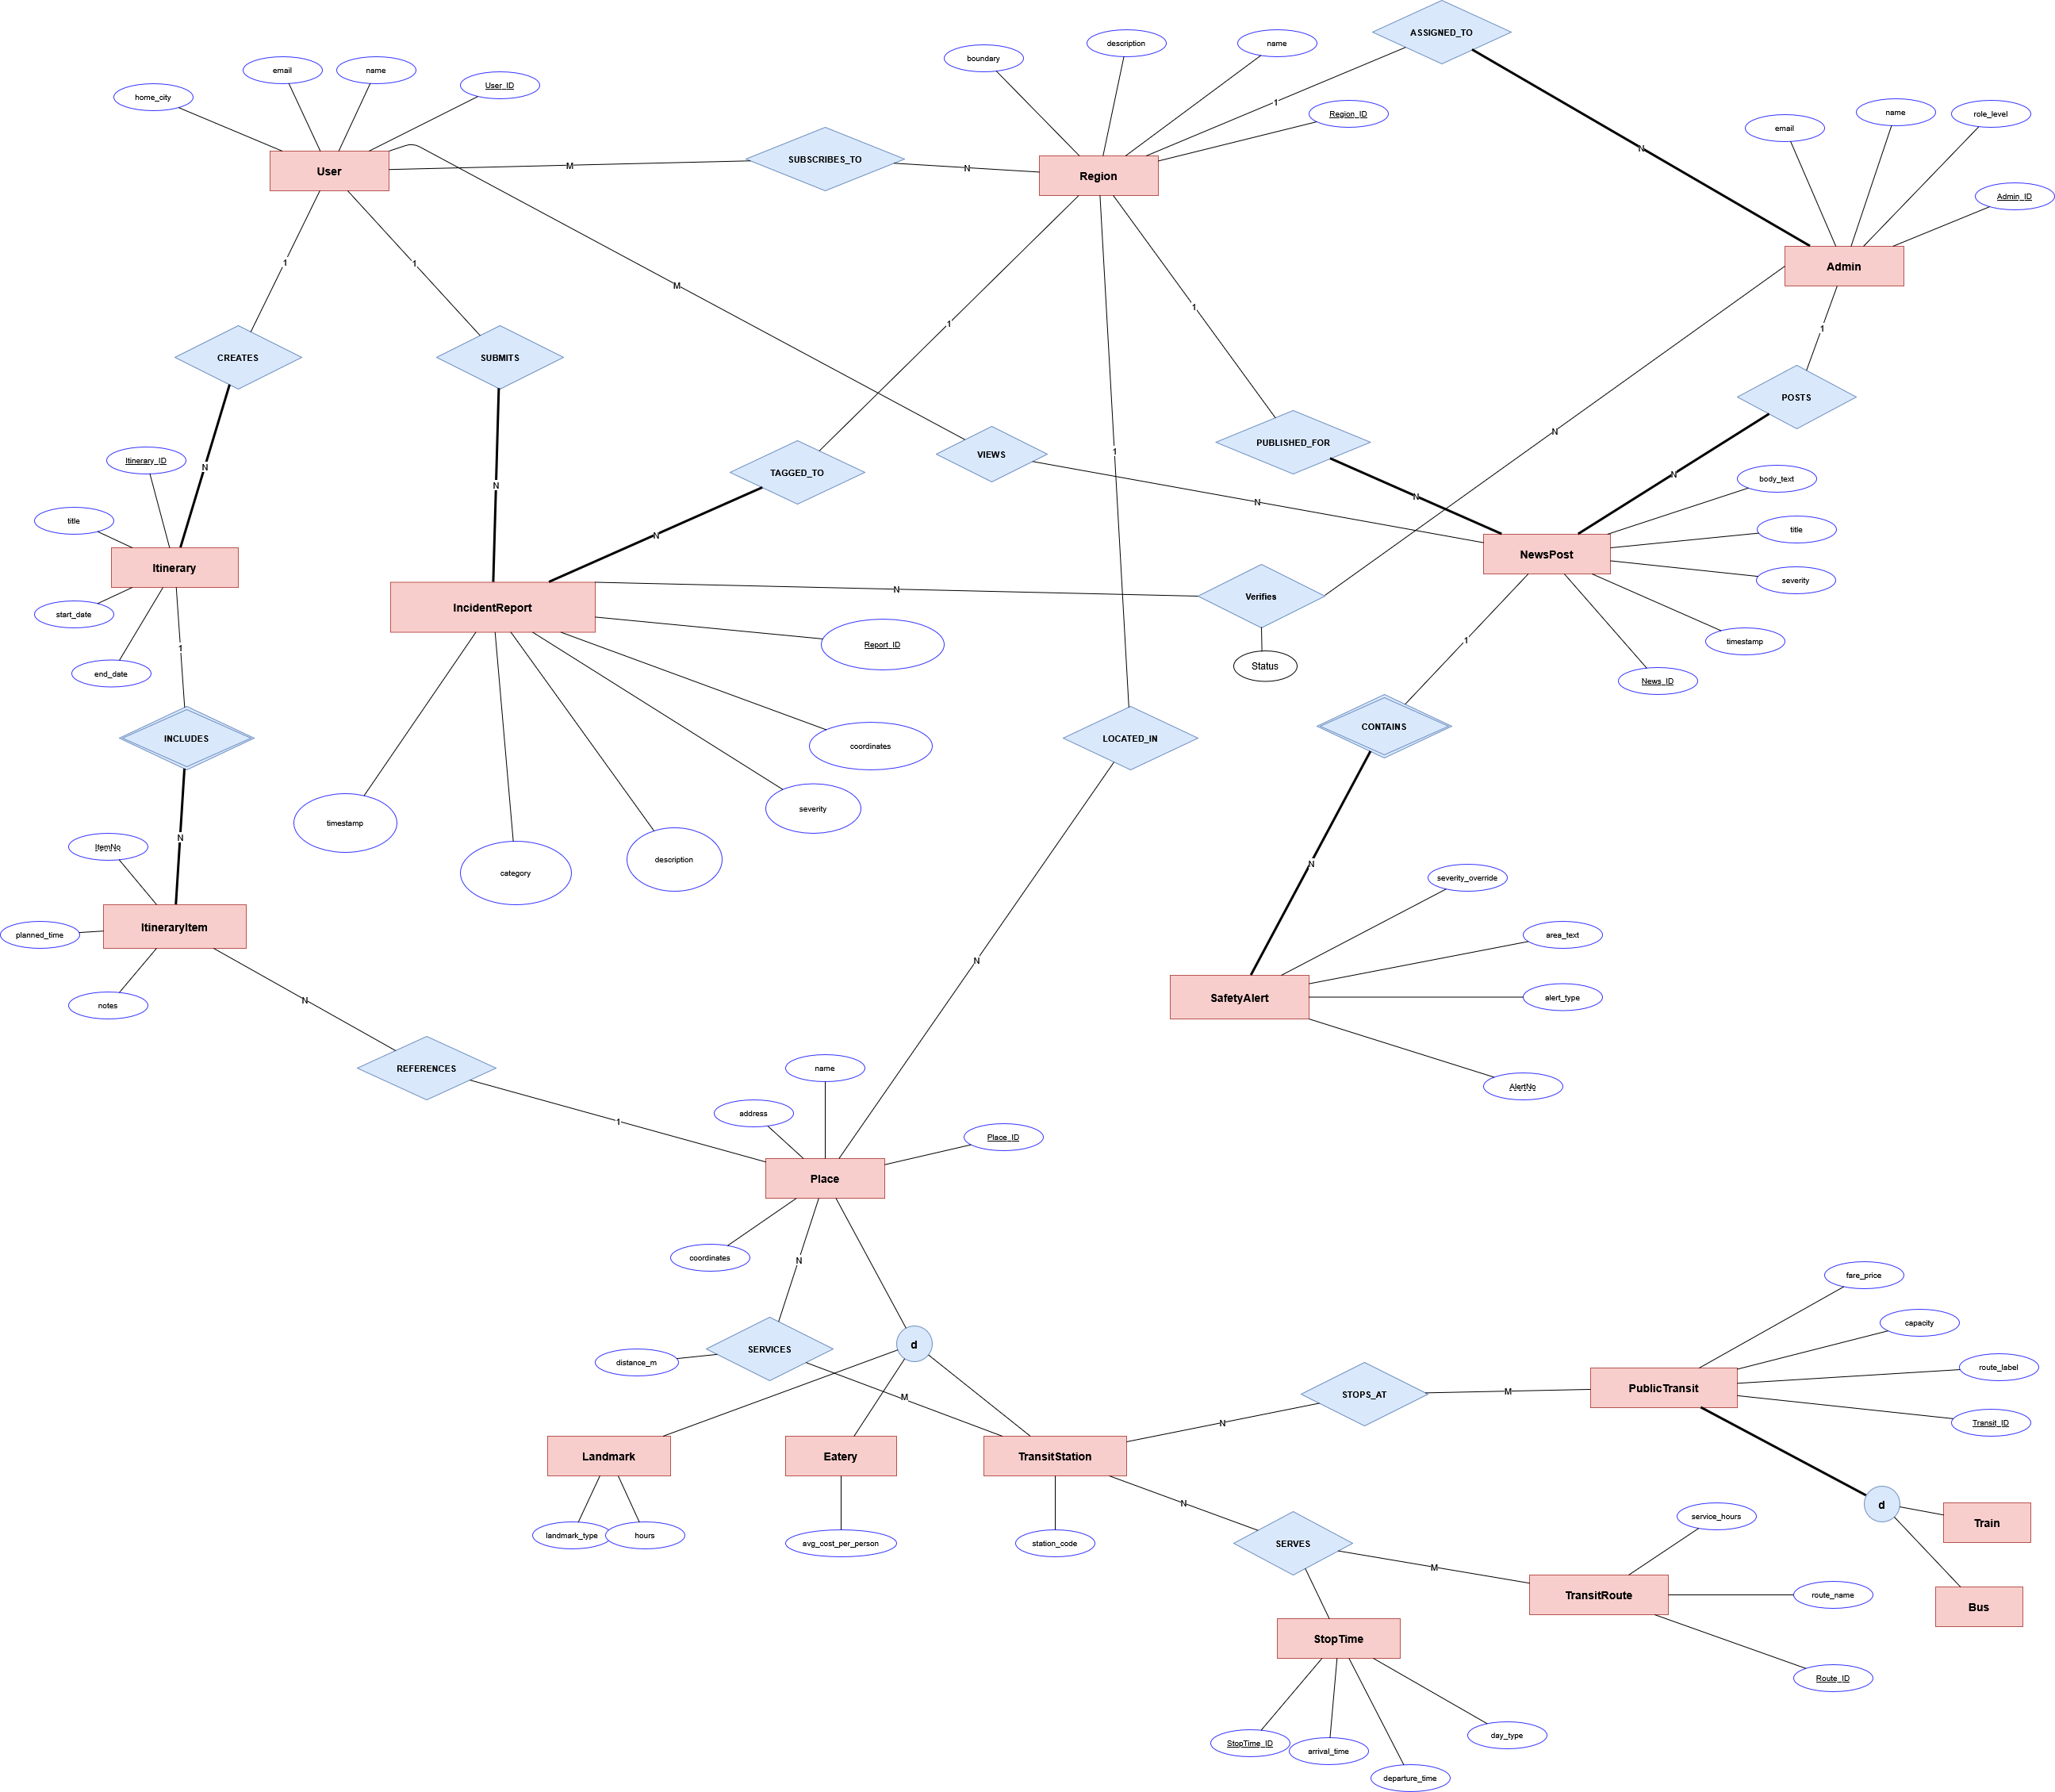
\includegraphics[width=\textwidth,keepaspectratio]{figures/eer.png}%
    }{%
        \fbox{\parbox{0.95\textwidth}{\centering\vspace{3cm}\textbf{Placeholder for EER diagram}\\\vspace{0.3cm}This figure will show the Extended Entity-Relationship diagram for Urban Scout, including all 16 entity types, the two specialization hierarchies (\texttt{Place} and \texttt{PublicTransit}), the two weak entities (\texttt{SafetyAlert} and \texttt{ItineraryItem}), and all relationship types.\\\vspace{0.3cm}\texttt{figures/eer.png}\vspace{3cm}}}%
    }
    \caption{Extended Entity-Relationship diagram for Urban Scout.}
    \label{fig:eer}
\end{figure}

No structural changes were made to the schema between the presentation and this final report. Features that were not yet wired up at presentation time, such as admin-side place management and admin-side transit route management, were already represented in the EER and only required interface implementation. The diagram above matches the version shown during the demo.

\subsection{Design Assumptions}

The following assumptions guided the conceptual and relational design of Urban Scout. They clarify how the schema enforces identity, participation, and referential constraints across the major entities.

\begin{enumerate}
    \item \texttt{USER(UserID)} uniquely identifies each user account.
    \item \texttt{ADMIN(AdminID)} uniquely identifies each admin.
    \item Admins are the only entities referenced by \texttt{NEWS\_POST.AdminID}, enforcing that only admins can create news content.
    \item Each \texttt{ADMIN} tuple contains a foreign key \texttt{RegionID} referencing \texttt{REGION(RegionID)}, enforcing that each admin is assigned to exactly one region and that admins can only manage content for their assigned region.
    \item \texttt{PLACE(PlaceID)} uniquely identifies each place.
    \item \texttt{PLACE} contains a foreign key \texttt{RegionID} referencing \texttt{REGION(RegionID)}, enforcing that each place belongs to exactly one region and cannot belong to multiple regions.
    \item The specialization of \texttt{PLACE} into \texttt{LANDMARK}, \texttt{EATERY}, and \texttt{TRANSIT\_STATION} is disjoint and partial. Disjoint means a given \texttt{PlaceID} can appear in at most one subclass table. Partial means a \texttt{PlaceID} may exist in \texttt{PLACE} without appearing in any subclass relation.
    \item Each subclass relation (\texttt{LANDMARK}, \texttt{EATERY}, \texttt{TRANSIT\_STATION}) uses \texttt{PlaceID} as both its primary key and a foreign key referencing \texttt{PLACE(PlaceID)}.
    \item \texttt{NEWS\_POST(NewsID)} uniquely identifies each news post.
    \item \texttt{NEWS\_POST.RegionID} is a foreign key referencing \texttt{REGION(RegionID)}, enforcing that each news post is published for exactly one region while a region may have multiple news posts.
    \item \texttt{SAFETY\_ALERT} is a weak entity. It is identified by the composite primary key \texttt{(NewsID, AlertNo)}, where \texttt{NewsID} is a foreign key referencing \texttt{NEWS\_POST(NewsID)}. Total participation is enforced because \texttt{NewsID} is part of the primary key and cannot be null.
    \item \texttt{INCIDENT\_REPORT(Report\_ID)} uniquely identifies each incident report.
    \item \texttt{INCIDENT\_REPORT.UserID} is a foreign key referencing \texttt{USER(UserID)}, enforcing that each report is submitted by exactly one user while a user may submit multiple reports.
    \item \texttt{INCIDENT\_REPORT.RegionID} is a foreign key referencing \texttt{REGION(RegionID)}, enforcing that each report is associated with exactly one region while a region may have multiple reports.
    \item The many-to-many relationship between \texttt{USER} and \texttt{REGION} is resolved by \texttt{SUBSCRIPTION(UserID, RegionID)}, which uses a composite primary key where both attributes are foreign keys referencing their respective parent relations.
    \item \texttt{TRANSIT\_ROUTE(RouteID)} uniquely identifies each transit route.
    \item \texttt{STOP\_TIME(RouteID, PlaceID, arrival\_time)} has a composite primary key. \texttt{RouteID} references \texttt{TRANSIT\_ROUTE(RouteID)} and \texttt{PlaceID} references \texttt{TRANSIT\_STATION(PlaceID)}. The relation also stores schedule attributes such as \texttt{arrival\_time}, \texttt{departure\_time}, and \texttt{sequence\_number}.
    \item Transit station to place proximity is modeled as a stored relationship attribute (for example, \texttt{walking\_distance}) and does not require a separate associative relation.
    \item All foreign key attributes enforce referential integrity constraints. A foreign key value must reference an existing primary key value, and primary key attributes cannot be null.
\end{enumerate}

\subsection{Design Rationale}

The final design reflects a balance between realism and project scope. The system is complex enough to demonstrate meaningful database concepts such as specialization, weak entities, role-based users, and many-to-many relationships, but still focused enough to be implemented within a course project. The schema was designed not only to satisfy database design requirements, but also to support visible frontend functionality.

As a result, Urban Scout is more than a collection of unrelated tables. It is a relational system in which data about places, transit, alerts, reports, and travel plans can be combined to support a coherent user experience.

\section{Implementation}
\nopagebreak[4]
\subsection{Relational Model Overview}

After the conceptual design was finalized through the ER diagram, the next step was to convert that design into a relational schema suitable for implementation in a relational DBMS. The resulting schema was designed to preserve the structure of the conceptual model while supporting the application features required by Urban Scout.

The implementation includes relations for users, administrators, regions, places, specialized place types, transit services, transit routes, news posts, safety alerts, incident reports, itineraries, and associative relationships connecting those entities. The schema reflects the standard transformation process from entity-relationship design to a relational model. Strong entities became base relations, specialization was implemented through subtype tables, weak entities were converted using composite keys, and many-to-many relationships were represented through linking tables.

The final relational structure supports both the frontend interface and backend endpoints. Each table has a clear role in storing core data or representing relationships between entities, which allows the system to retrieve connected information efficiently. The relational schema and UML class diagrams (Figures~\ref{fig:rm} and~\ref{fig:uml}) illustrate the full set of tables and their relationships.

\begin{figure}[p]
    \centering
    \IfFileExists{figures/relational-model.png}{%
        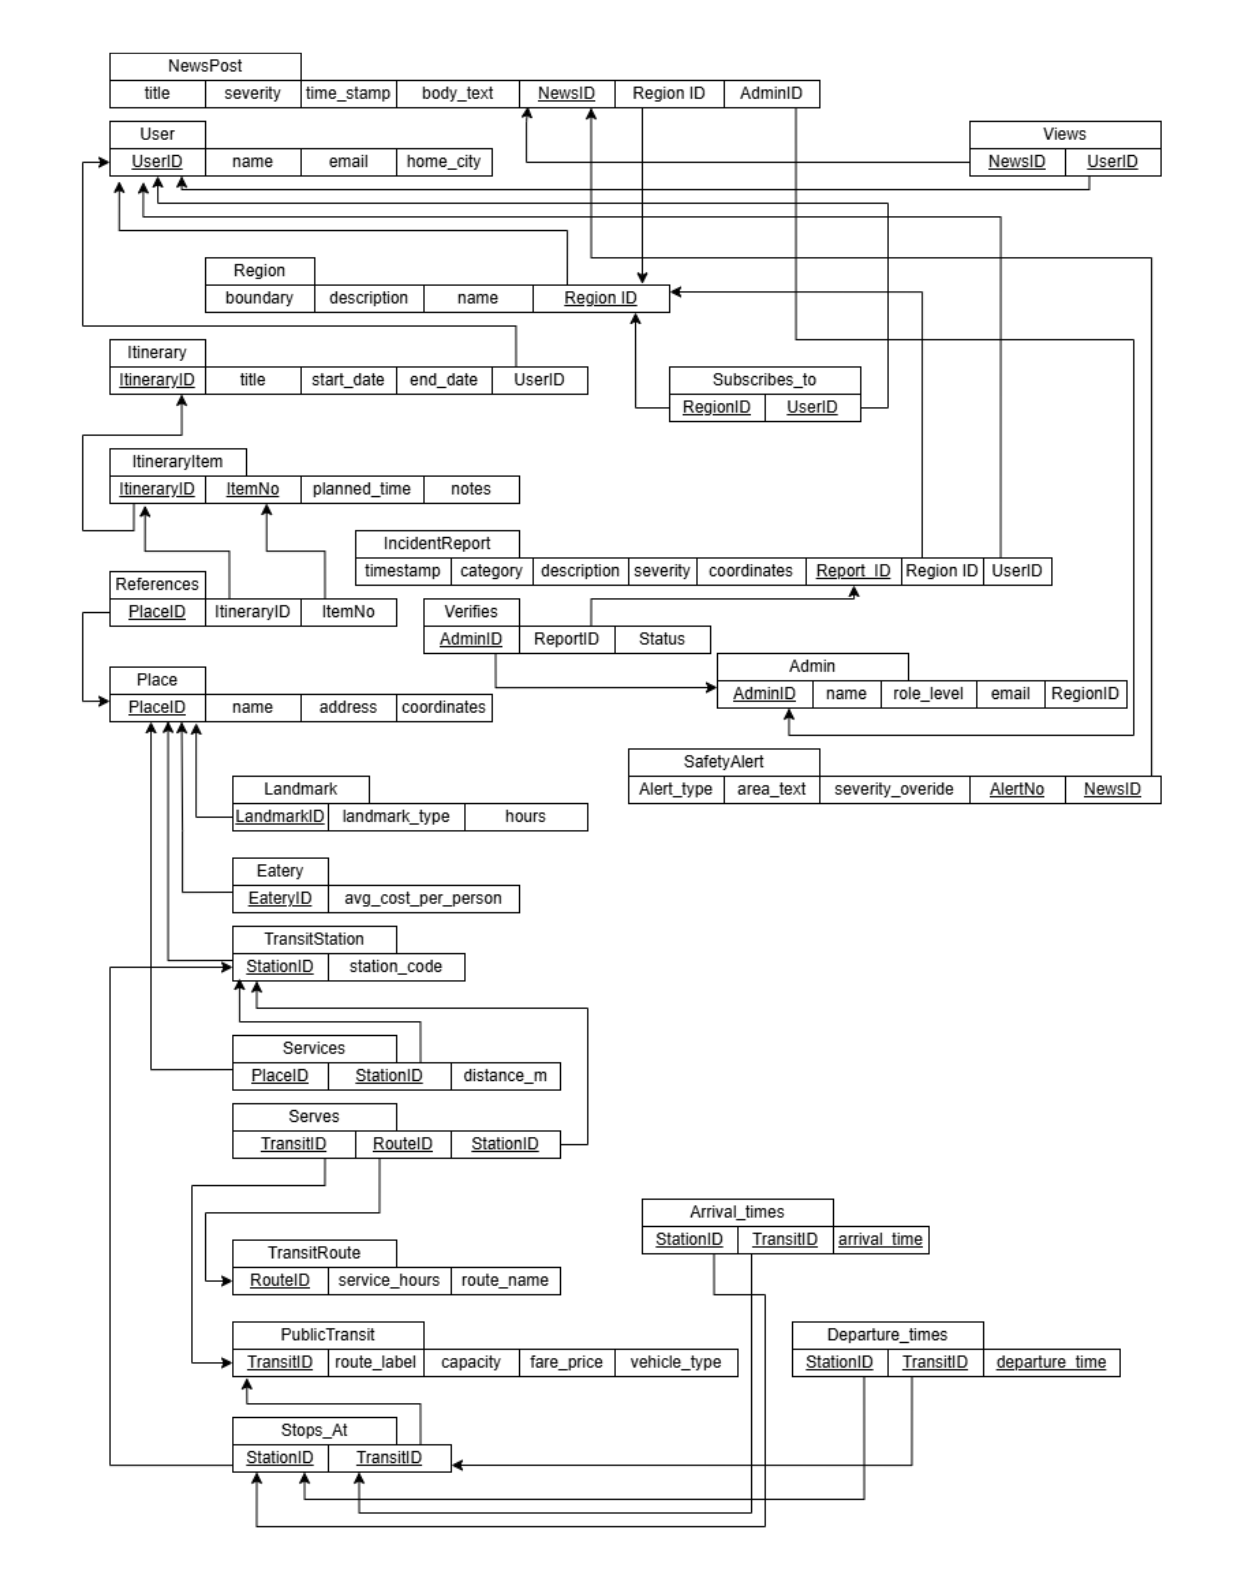
\includegraphics[width=\textwidth,height=0.9\textheight,keepaspectratio]{figures/relational-model.png}%
    }{%
        \fbox{\parbox{0.95\textwidth}{\centering\vspace{3cm}\textbf{Placeholder for Relational Model diagram}\\\vspace{0.3cm}This figure will show the relational schema diagram for Urban Scout, derived from the EER through the standard mapping algorithm. It will include all 25 tables with primary and foreign key relationships drawn out.\\\vspace{0.3cm}\texttt{figures/relational-model.png}\vspace{3cm}}}%
    }
    \caption{Relational schema diagram for Urban Scout.}
    \label{fig:rm}
\end{figure}

\begin{figure}[p]
    \centering
    \IfFileExists{figures/uml.png}{%
        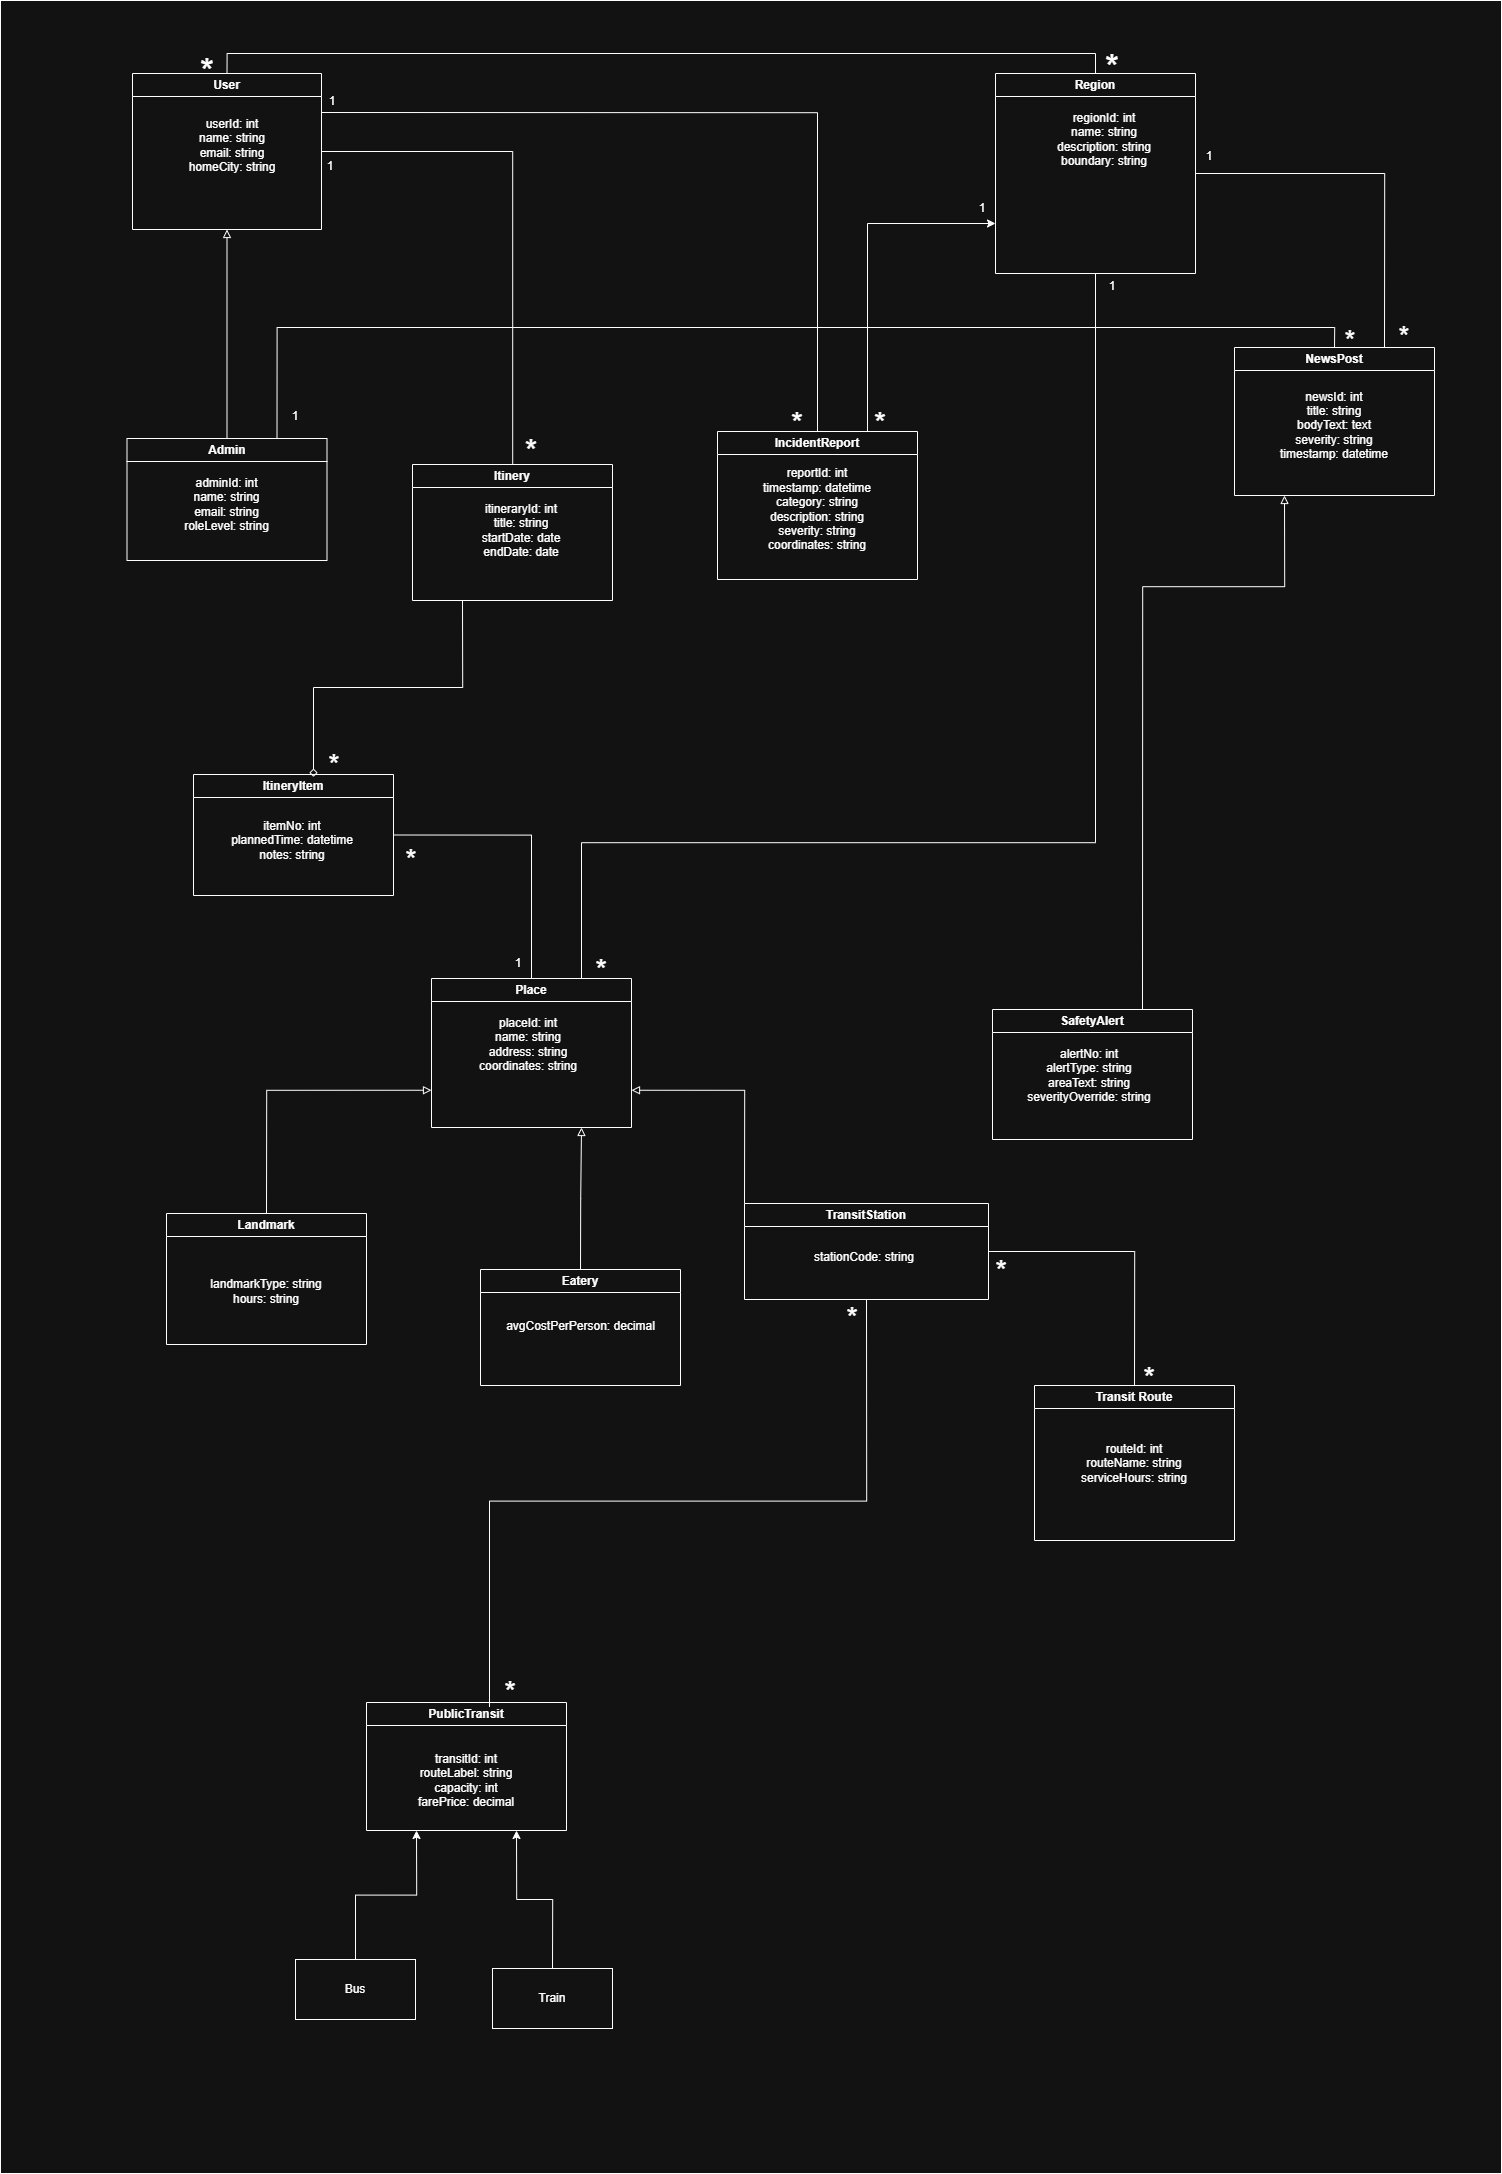
\includegraphics[width=\textwidth,height=0.9\textheight,keepaspectratio]{figures/uml.png}%
    }{%
        \fbox{\parbox{0.95\textwidth}{\centering\vspace{3cm}\textbf{Placeholder for UML class diagram}\\\vspace{0.3cm}This figure will show the UML class diagram for the Urban Scout relational model, displaying all entity classes with their attributes and inter-table relationships.\\\vspace{0.3cm}\texttt{figures/uml.png}\vspace{3cm}}}%
    }
    \caption{UML class diagram showing entity attributes and relationships.}
    \label{fig:uml}
\end{figure}

\subsection{Conversion from ER Diagram to Relational Schema}

The relational schema was created by following the standard ER-to-relational mapping approach.

\boldheading{Strong Entities}

Strong entities in the ER diagram were mapped directly into tables with primary keys. Examples include \texttt{User}, \texttt{Admin}, \texttt{Region}, \texttt{Place}, \texttt{TransitRoute}, \texttt{PublicTransit}, \texttt{NewsPost}, \texttt{IncidentReport}, and \texttt{Itinerary}. Each of these relations has its own primary key and stores attributes that belong directly to that entity.

\boldheading{Specialization}

One of the important design decisions in the project was the specialization of \texttt{Place} into \texttt{Landmark}, \texttt{Eatery}, and \texttt{TransitStation}. Instead of storing all place-specific attributes in a single large table, the implementation uses separate subtype tables. \texttt{Place} stores shared attributes such as name, address, coordinates, and region. \texttt{Landmark} stores landmark-specific data, \texttt{Eatery} stores eatery-specific data, and \texttt{TransitStation} stores station-specific data.

This design was chosen because it keeps the database normalized and avoids storing many null attributes in a single universal place table. It also reflects the conceptual distinction between different kinds of locations while preserving their shared identity.

\boldheading{Weak Entities}

Two important weak entities appear in the schema: \texttt{SafetyAlert} and \texttt{ItineraryItem}. \texttt{SafetyAlert} depends on \texttt{NewsPost}, so it was implemented with a composite key including the owning news post identifier and a local alert number. \texttt{ItineraryItem} depends on \texttt{Itinerary}, so it was implemented with a composite key including the itinerary identifier and an item number.

The use of weak entities was an important part of the project because it allowed the schema to represent dependent data in a structured and relationally correct way.

\boldheading{Many-to-Many Relationships}

Several many-to-many relationships in the ER diagram were converted into separate associative tables. These include user subscriptions to regions, itinerary items referencing places, routes serving stations through transit services, places being near transit stations, users viewing news posts, and administrators verifying incident reports.

These relationships were implemented through linking tables such as \texttt{Subscribes\_to}, \texttt{References}, \texttt{Serves}, \texttt{Services}, \texttt{Views}, and \texttt{Verifies}. This decision was necessary because many-to-many relationships cannot be represented directly in a normalized relational schema without introducing a separate relation.

\subsection{Significant Design Decisions}

Several implementation decisions were especially important during the conversion process.

\boldheading{Use of Separate Admin and User Tables}

The project keeps \texttt{User} and \texttt{Admin} as separate tables rather than placing both roles into one shared account table. This was done to keep the distinction between tourists and administrators explicit in both the schema and the application logic. Because the two user types have different roles and responsibilities, separating them simplified access control and role-based routing in the backend.

\boldheading{Modeling Transit with Multiple Related Tables}

Transit information was not stored in a single table. Instead, the design separates transit services (\texttt{PublicTransit}), route information (\texttt{TransitRoute}), stations (\texttt{TransitStation}), station-route-service relationships (\texttt{Serves}), stop relationships (\texttt{Stops\_At}), and arrival and departure schedules (\texttt{Arrival\_times}, \texttt{Departure\_times}).

This decision increased the complexity of the schema, but it allowed the project to model the transit system in a much more realistic way. It also supported one of the project's showcase queries: retrieving the full schedule and service information for a selected station.

\boldheading{Region-Centered Organization}

Another major implementation choice was to make \texttt{Region} a central organizing entity. Instead of treating the city as a single undifferentiated space, the schema uses regions to group places, news, subscriptions, reports, and administrative responsibilities. This makes filtering and personalization much easier in the application.

\subsection{DBMS Selection}

The project was implemented using \textbf{MySQL} as the DBMS.

MySQL was selected for several reasons:
\begin{itemize}
    \item it is a widely used relational database system
    \item it aligns well with the course focus on SQL and relational database design
    \item it supports foreign keys, joins, procedures, and indexing features needed for the project
    \item it integrates smoothly with the Node.js backend using the \texttt{mysql2} library
    \item it is accessible and practical for local development and demonstration
\end{itemize}

Because the project emphasizes database concepts, MySQL was an appropriate choice. It allowed the team to implement the schema directly in SQL and demonstrate clear understanding of relational modeling, rather than relying on an abstraction layer such as an ORM.

\subsection{Database Implementation}

The database implementation was organized through SQL scripts that define the schema, insert sample data, and create stored procedures.

The implementation includes:
\begin{itemize}
    \item a schema script to create all relations and constraints
    \item a seed script to populate the database with sample data
    \item a script for stored procedures
    \item a drop/reset script used during testing and redevelopment
\end{itemize}
\nopagebreak[4]

\noindent This structure made the project easier to maintain and reset during development. It also ensured that the same database could be recreated consistently for testing, demo preparation, and final submission.

\boldheading{Schema Definition (DDL)}

\begin{lstlisting}[language=MySQL,caption={Full database schema (DDL).},label={lst:ddl}]
-- Urban Scout - CPSC 471 Group 61 - Database Schema (MySQL 8.0)

CREATE DATABASE IF NOT EXISTS UrbanScout;
USE UrbanScout;

CREATE TABLE User (
    UserID      INT             PRIMARY KEY AUTO_INCREMENT,
    name        VARCHAR(100)    NOT NULL,
    email       VARCHAR(150)    NOT NULL UNIQUE,
    home_city   VARCHAR(100)
);

CREATE TABLE Region (
    RegionID    INT             PRIMARY KEY AUTO_INCREMENT,
    name        VARCHAR(100)    NOT NULL,
    description TEXT,
    boundary    VARCHAR(255)
);

CREATE TABLE Admin (
    AdminID     INT             PRIMARY KEY AUTO_INCREMENT,
    name        VARCHAR(100)    NOT NULL,
    email       VARCHAR(150)    NOT NULL UNIQUE,
    role_level  VARCHAR(50),
    RegionID    INT             NOT NULL,
    FOREIGN KEY (RegionID) REFERENCES Region(RegionID)
        ON DELETE RESTRICT ON UPDATE CASCADE
);

CREATE TABLE Place (
    PlaceID     INT             PRIMARY KEY AUTO_INCREMENT,
    name        VARCHAR(150)    NOT NULL,
    address     VARCHAR(255),
    coordinates VARCHAR(50),
    RegionID    INT             NOT NULL,
    FOREIGN KEY (RegionID) REFERENCES Region(RegionID)
        ON DELETE RESTRICT ON UPDATE CASCADE
);

CREATE TABLE Landmark (
    LandmarkID      INT         PRIMARY KEY,
    landmark_type   VARCHAR(50),
    hours           VARCHAR(100),
    FOREIGN KEY (LandmarkID) REFERENCES Place(PlaceID)
        ON DELETE CASCADE ON UPDATE CASCADE
);

CREATE TABLE Eatery (
    EateryID            INT             PRIMARY KEY,
    avg_cost_per_person DECIMAL(8,2),
    FOREIGN KEY (EateryID) REFERENCES Place(PlaceID)
        ON DELETE CASCADE ON UPDATE CASCADE
);

CREATE TABLE TransitStation (
    StationID       INT         PRIMARY KEY,
    station_code    VARCHAR(20),
    FOREIGN KEY (StationID) REFERENCES Place(PlaceID)
        ON DELETE CASCADE ON UPDATE CASCADE
);

CREATE TABLE TransitRoute (
    RouteID         INT             PRIMARY KEY AUTO_INCREMENT,
    route_name      VARCHAR(100)    NOT NULL,
    service_hours   VARCHAR(100)
);

CREATE TABLE PublicTransit (
    TransitID       INT             PRIMARY KEY AUTO_INCREMENT,
    route_label     VARCHAR(50),
    capacity        INT,
    fare_price      DECIMAL(6,2),
    vehicle_type    VARCHAR(20)
);

CREATE TABLE Bus (
    TransitID       INT         PRIMARY KEY,
    bus_number      VARCHAR(20),
    FOREIGN KEY (TransitID) REFERENCES PublicTransit(TransitID)
        ON DELETE CASCADE ON UPDATE CASCADE
);

CREATE TABLE Train (
    TransitID       INT         PRIMARY KEY,
    car_count       INT,
    FOREIGN KEY (TransitID) REFERENCES PublicTransit(TransitID)
        ON DELETE CASCADE ON UPDATE CASCADE
);

CREATE TABLE NewsPost (
    NewsID      INT             PRIMARY KEY AUTO_INCREMENT,
    title       VARCHAR(200)    NOT NULL,
    severity    VARCHAR(20),
    time_stamp  DATETIME        NOT NULL DEFAULT CURRENT_TIMESTAMP,
    body_text   TEXT,
    RegionID    INT             NOT NULL,
    AdminID     INT             NOT NULL,
    FOREIGN KEY (RegionID) REFERENCES Region(RegionID)
        ON DELETE RESTRICT ON UPDATE CASCADE,
    FOREIGN KEY (AdminID) REFERENCES Admin(AdminID)
        ON DELETE RESTRICT ON UPDATE CASCADE
);

CREATE TABLE SafetyAlert (
    NewsID              INT             NOT NULL,
    AlertNo             INT             NOT NULL,
    alert_type          VARCHAR(50),
    area_text           VARCHAR(255),
    severity_override   VARCHAR(20),
    PRIMARY KEY (NewsID, AlertNo),
    FOREIGN KEY (NewsID) REFERENCES NewsPost(NewsID)
        ON DELETE CASCADE ON UPDATE CASCADE
);

CREATE TABLE IncidentReport (
    Report_ID   INT             PRIMARY KEY AUTO_INCREMENT,
    timestamp   DATETIME        NOT NULL DEFAULT CURRENT_TIMESTAMP,
    category    VARCHAR(50),
    description TEXT,
    severity    VARCHAR(20),
    coordinates VARCHAR(50),
    UserID      INT             NOT NULL,
    RegionID    INT             NOT NULL,
    FOREIGN KEY (UserID) REFERENCES User(UserID)
        ON DELETE CASCADE ON UPDATE CASCADE,
    FOREIGN KEY (RegionID) REFERENCES Region(RegionID)
        ON DELETE RESTRICT ON UPDATE CASCADE
);

CREATE TABLE Itinerary (
    ItineraryID INT             PRIMARY KEY AUTO_INCREMENT,
    title       VARCHAR(150)    NOT NULL,
    start_date  DATE,
    end_date    DATE,
    UserID      INT             NOT NULL,
    FOREIGN KEY (UserID) REFERENCES User(UserID)
        ON DELETE CASCADE ON UPDATE CASCADE
);

CREATE TABLE ItineraryItem (
    ItineraryID INT         NOT NULL,
    ItemNo      INT         NOT NULL,
    planned_time DATETIME,
    notes       TEXT,
    PRIMARY KEY (ItineraryID, ItemNo),
    FOREIGN KEY (ItineraryID) REFERENCES Itinerary(ItineraryID)
        ON DELETE CASCADE ON UPDATE CASCADE
);

CREATE TABLE `References` (
    PlaceID     INT     NOT NULL,
    ItineraryID INT     NOT NULL,
    ItemNo      INT     NOT NULL,
    PRIMARY KEY (PlaceID, ItineraryID, ItemNo),
    FOREIGN KEY (PlaceID)       REFERENCES Place(PlaceID)
        ON DELETE CASCADE ON UPDATE CASCADE,
    FOREIGN KEY (ItineraryID, ItemNo) REFERENCES ItineraryItem(ItineraryID, ItemNo)
        ON DELETE CASCADE ON UPDATE CASCADE
);

CREATE TABLE Subscribes_to (
    UserID      INT     NOT NULL,
    RegionID    INT     NOT NULL,
    PRIMARY KEY (UserID, RegionID),
    FOREIGN KEY (UserID)    REFERENCES User(UserID)
        ON DELETE CASCADE ON UPDATE CASCADE,
    FOREIGN KEY (RegionID)  REFERENCES Region(RegionID)
        ON DELETE CASCADE ON UPDATE CASCADE
);

CREATE TABLE Views (
    UserID  INT     NOT NULL,
    NewsID  INT     NOT NULL,
    PRIMARY KEY (UserID, NewsID),
    FOREIGN KEY (UserID) REFERENCES User(UserID)
        ON DELETE CASCADE ON UPDATE CASCADE,
    FOREIGN KEY (NewsID) REFERENCES NewsPost(NewsID)
        ON DELETE CASCADE ON UPDATE CASCADE
);

CREATE TABLE Verifies (
    AdminID     INT             NOT NULL,
    ReportID    INT             NOT NULL,
    Status      VARCHAR(30)     NOT NULL DEFAULT 'pending',
    PRIMARY KEY (AdminID, ReportID),
    FOREIGN KEY (AdminID)   REFERENCES Admin(AdminID)
        ON DELETE CASCADE ON UPDATE CASCADE,
    FOREIGN KEY (ReportID)  REFERENCES IncidentReport(Report_ID)
        ON DELETE CASCADE ON UPDATE CASCADE
);

CREATE TABLE Services (
    PlaceID     INT             NOT NULL,
    StationID   INT             NOT NULL,
    distance_m  DECIMAL(8,1),
    PRIMARY KEY (PlaceID, StationID),
    FOREIGN KEY (PlaceID)   REFERENCES Place(PlaceID)
        ON DELETE CASCADE ON UPDATE CASCADE,
    FOREIGN KEY (StationID) REFERENCES TransitStation(StationID)
        ON DELETE CASCADE ON UPDATE CASCADE
);

CREATE TABLE Serves (
    RouteID     INT     NOT NULL,
    StationID   INT     NOT NULL,
    TransitID   INT     NOT NULL,
    PRIMARY KEY (RouteID, StationID, TransitID),
    FOREIGN KEY (RouteID)   REFERENCES TransitRoute(RouteID)
        ON DELETE CASCADE ON UPDATE CASCADE,
    FOREIGN KEY (StationID) REFERENCES TransitStation(StationID)
        ON DELETE CASCADE ON UPDATE CASCADE,
    FOREIGN KEY (TransitID) REFERENCES PublicTransit(TransitID)
        ON DELETE CASCADE ON UPDATE CASCADE
);

CREATE TABLE Stops_At (
    StationID   INT     NOT NULL,
    TransitID   INT     NOT NULL,
    PRIMARY KEY (StationID, TransitID),
    FOREIGN KEY (StationID) REFERENCES TransitStation(StationID)
        ON DELETE CASCADE ON UPDATE CASCADE,
    FOREIGN KEY (TransitID) REFERENCES PublicTransit(TransitID)
        ON DELETE CASCADE ON UPDATE CASCADE
);

CREATE TABLE Arrival_times (
    TransitID       INT     NOT NULL,
    StationID       INT     NOT NULL,
    arrival_time    TIME    NOT NULL,
    PRIMARY KEY (TransitID, StationID, arrival_time),
    FOREIGN KEY (TransitID) REFERENCES PublicTransit(TransitID)
        ON DELETE CASCADE ON UPDATE CASCADE,
    FOREIGN KEY (StationID) REFERENCES TransitStation(StationID)
        ON DELETE CASCADE ON UPDATE CASCADE
);

CREATE TABLE Departure_times (
    TransitID       INT     NOT NULL,
    StationID       INT     NOT NULL,
    departure_time  TIME    NOT NULL,
    PRIMARY KEY (TransitID, StationID, departure_time),
    FOREIGN KEY (TransitID) REFERENCES PublicTransit(TransitID)
        ON DELETE CASCADE ON UPDATE CASCADE,
    FOREIGN KEY (StationID) REFERENCES TransitStation(StationID)
        ON DELETE CASCADE ON UPDATE CASCADE
);
\end{lstlisting}

\subsection{Transactions and SQL Statements}

The application exposes 36 REST endpoints across 8 route modules. Each endpoint maps to one or more SQL statements that are executed using \texttt{mysql2} prepared statements. The complete list grouped by feature area follows below.

\subsubsection{Authentication}

\textbf{POST /api/auth/register} \textit{(Auth: none.)}
Creates a new user account and saves the user to the session.
\begin{lstlisting}[language=MySQL]
INSERT INTO User (name, email, home_city) VALUES (?, ?, ?);
\end{lstlisting}

\textbf{POST /api/auth/login} \textit{(Auth: none.)}
Looks up a user by email and establishes a session.
\begin{lstlisting}[language=MySQL]
SELECT * FROM User WHERE email = ?;
\end{lstlisting}

\textbf{POST /api/auth/admin-login} \textit{(Auth: none.)}
Looks up an admin by email and establishes an admin session.
\begin{lstlisting}[language=MySQL]
SELECT * FROM Admin WHERE email = ?;
\end{lstlisting}

\textbf{POST /api/auth/logout} \textit{(Auth: none.)}
Destroys the current session.
\textit{No SQL is executed. The handler only clears the session.}

\textbf{GET /api/auth/me} \textit{(Auth: none.)}
Returns the currently logged-in user or admin, or null if no session is active.
\textit{No SQL is executed. The handler only inspects the session.}

\subsubsection{Regions}

\textbf{GET /api/regions} \textit{(Auth: none.)}
Retrieves all regions for the home page.
\begin{lstlisting}[language=MySQL]
SELECT * FROM Region;
\end{lstlisting}

\textbf{GET /api/regions/:id} \textit{(Auth: none.)}
Retrieves a single region together with its place count and news post count.
\begin{lstlisting}[language=MySQL]
SELECT * FROM Region WHERE RegionID = ?;
SELECT COUNT(*) as count FROM Place WHERE RegionID = ?;
SELECT COUNT(*) as count FROM NewsPost WHERE RegionID = ?;
\end{lstlisting}

\subsubsection{Places}

\textbf{GET /api/places} \textit{(Auth: none.)}
Retrieves all places, optionally filtered by region and place type. The handler picks one of four query branches based on the type parameter.
\begin{lstlisting}[language=MySQL]
-- when type=landmark
SELECT p.*, l.landmark_type, l.hours
FROM Place p JOIN Landmark l ON p.PlaceID = l.LandmarkID
WHERE 1=1 ORDER BY p.name;

-- when type=eatery
SELECT p.*, e.avg_cost_per_person
FROM Place p JOIN Eatery e ON p.PlaceID = e.EateryID
WHERE 1=1 ORDER BY p.name;

-- when type=transit
SELECT p.*, ts.station_code
FROM Place p JOIN TransitStation ts ON p.PlaceID = ts.StationID
WHERE 1=1 ORDER BY p.name;

-- when no type filter
SELECT p.*,
  CASE
    WHEN l.LandmarkID IS NOT NULL THEN 'landmark'
    WHEN e.EateryID IS NOT NULL THEN 'eatery'
    WHEN ts.StationID IS NOT NULL THEN 'transit'
    ELSE 'other'
  END AS placeType,
  l.landmark_type, l.hours,
  e.avg_cost_per_person,
  ts.station_code
FROM Place p
LEFT JOIN Landmark l ON p.PlaceID = l.LandmarkID
LEFT JOIN Eatery e ON p.PlaceID = e.EateryID
LEFT JOIN TransitStation ts ON p.PlaceID = ts.StationID
WHERE 1=1 ORDER BY p.name;

-- regionId filter appended:
-- AND p.RegionID = ?
\end{lstlisting}

\textbf{GET /api/places/:id} \textit{(Auth: none.)}
Retrieves a single place along with its specialization details and any nearby transit stations.
\begin{lstlisting}[language=MySQL]
SELECT p.*,
  l.landmark_type, l.hours,
  e.avg_cost_per_person,
  ts.station_code,
  CASE
    WHEN l.LandmarkID IS NOT NULL THEN 'landmark'
    WHEN e.EateryID IS NOT NULL THEN 'eatery'
    WHEN ts.StationID IS NOT NULL THEN 'transit'
    ELSE 'other'
  END AS placeType
FROM Place p
LEFT JOIN Landmark l ON p.PlaceID = l.LandmarkID
LEFT JOIN Eatery e ON p.PlaceID = e.EateryID
LEFT JOIN TransitStation ts ON p.PlaceID = ts.StationID
WHERE p.PlaceID = ?;

SELECT s.distance_m, p.name AS station_name, ts.station_code, p.PlaceID AS StationPlaceID
FROM Services s
JOIN Place p ON s.StationID = p.PlaceID
JOIN TransitStation ts ON s.StationID = ts.StationID
WHERE s.PlaceID = ?
ORDER BY s.distance_m ASC;
\end{lstlisting}

\textbf{POST /api/places} \textit{(Auth: admin.)}
Creates a new place along with its specialization row inside a single transaction so the parent and subtype rows stay in sync.
\begin{lstlisting}[language=MySQL]
START TRANSACTION;

INSERT INTO Place (name, address, coordinates, RegionID)
VALUES (?, ?, ?, ?);

-- one of the following depending on type
INSERT INTO Landmark (LandmarkID, landmark_type, hours) VALUES (?, ?, ?);
INSERT INTO Eatery (EateryID, avg_cost_per_person) VALUES (?, ?);
INSERT INTO TransitStation (StationID, station_code) VALUES (?, ?);

COMMIT;
\end{lstlisting}

\subsubsection{Transit}

\textbf{GET /api/transit/routes} \textit{(Auth: none.)}
Retrieves all transit routes.
\begin{lstlisting}[language=MySQL]
SELECT * FROM TransitRoute;
\end{lstlisting}

\textbf{POST /api/transit/routes} \textit{(Auth: admin.)}
Adds a new transit route.
\begin{lstlisting}[language=MySQL]
INSERT INTO TransitRoute (route_name, service_hours) VALUES (?, ?);
\end{lstlisting}

\textbf{DELETE /api/transit/routes/:id} \textit{(Auth: admin.)}
Deletes a transit route. The deletion cascades to the \texttt{Serves} junction table.
\begin{lstlisting}[language=MySQL]
DELETE FROM TransitRoute WHERE RouteID = ?;
\end{lstlisting}

\textbf{POST /api/transit/routes/:id/stations} \textit{(Auth: admin.)}
Links a station and a transit vehicle to a route as a stop.
\begin{lstlisting}[language=MySQL]
INSERT INTO Serves (RouteID, StationID, TransitID) VALUES (?, ?, ?);
\end{lstlisting}

\textbf{DELETE /api/transit/routes/:id/stations} \textit{(Auth: admin.)}
Removes a stop from a route.
\begin{lstlisting}[language=MySQL]
DELETE FROM Serves WHERE RouteID = ? AND StationID = ? AND TransitID = ?;
\end{lstlisting}

\textbf{GET /api/transit/routes/:id/stations} \textit{(Auth: none.)}
Lists the stops on a single route, joining station and vehicle information for display.
\begin{lstlisting}[language=MySQL]
SELECT sv.StationID, sv.TransitID,
       p.name AS station_name, ts.station_code,
       pt.route_label, pt.vehicle_type
FROM Serves sv
JOIN TransitStation ts ON sv.StationID = ts.StationID
JOIN Place p ON ts.StationID = p.PlaceID
JOIN PublicTransit pt ON sv.TransitID = pt.TransitID
WHERE sv.RouteID = ?
ORDER BY p.name;
\end{lstlisting}

\textbf{GET /api/transit/vehicles} \textit{(Auth: none.)}
Lists transit vehicles, with an optional vehicle type filter.
\begin{lstlisting}[language=MySQL]
SELECT * FROM PublicTransit;
-- with type filter:
SELECT * FROM PublicTransit WHERE vehicle_type = ?;
\end{lstlisting}

\textbf{GET /api/transit/stations/:id/schedule} \textit{(Auth: none.)}
Returns four result sets that together make up a station's schedule view: station info, arrivals, departures, and the routes that serve the station.
\begin{lstlisting}[language=MySQL]
SELECT p.name, p.address, p.coordinates, ts.station_code
FROM Place p JOIN TransitStation ts ON p.PlaceID = ts.StationID
WHERE ts.StationID = ?;

SELECT at.arrival_time, pt.route_label, pt.vehicle_type, pt.TransitID
FROM Arrival_times at JOIN PublicTransit pt ON at.TransitID = pt.TransitID
WHERE at.StationID = ?
ORDER BY at.arrival_time;

SELECT dt.departure_time, pt.route_label, pt.vehicle_type, pt.TransitID
FROM Departure_times dt JOIN PublicTransit pt ON dt.TransitID = pt.TransitID
WHERE dt.StationID = ?
ORDER BY dt.departure_time;

SELECT DISTINCT tr.RouteID, tr.route_name, tr.service_hours
FROM Serves sv JOIN TransitRoute tr ON sv.RouteID = tr.RouteID
WHERE sv.StationID = ?;
\end{lstlisting}

\textbf{GET /api/transit/stations/:id/nearby} \textit{(Auth: none.)}
Finds places within walking distance of a station by calling the \texttt{sp\_nearby\_places} stored procedure.
\begin{lstlisting}[language=MySQL]
CALL sp_nearby_places(?, ?);
\end{lstlisting}

\subsubsection{News}

\textbf{GET /api/news} \textit{(Auth: none for public browse, but the session is consulted to filter by subscriptions when a user is logged in and no \texttt{regionId} is supplied.)}
Retrieves news posts together with embedded safety alerts. The handler picks one of three branches: a specific region, the logged-in user's subscribed regions, or all news.
\begin{lstlisting}[language=MySQL]
-- anonymous, all news
SELECT np.*, r.name AS region_name, a.name AS admin_name,
  sa.AlertNo, sa.alert_type, sa.area_text, sa.severity_override
FROM NewsPost np
JOIN Region r ON np.RegionID = r.RegionID
JOIN Admin a ON np.AdminID = a.AdminID
LEFT JOIN SafetyAlert sa ON np.NewsID = sa.NewsID
ORDER BY np.time_stamp DESC;

-- with regionId
... WHERE np.RegionID = ? ORDER BY np.time_stamp DESC;

-- logged-in user, no regionId, default to subscribed regions
... WHERE np.RegionID IN (
  SELECT RegionID FROM Subscribes_to WHERE UserID = ?
) ORDER BY np.time_stamp DESC;
\end{lstlisting}

\textbf{GET /api/news/:id} \textit{(Auth: none.)}
Retrieves a single news post and its safety alerts.
\begin{lstlisting}[language=MySQL]
SELECT np.*, r.name AS region_name, a.name AS admin_name
FROM NewsPost np
JOIN Region r ON np.RegionID = r.RegionID
JOIN Admin a ON np.AdminID = a.AdminID
WHERE np.NewsID = ?;

SELECT * FROM SafetyAlert WHERE NewsID = ?;
\end{lstlisting}

\textbf{POST /api/news} \textit{(Auth: admin.)}
Creates a news post and optionally attaches one safety alert.
\begin{lstlisting}[language=MySQL]
INSERT INTO NewsPost (title, severity, body_text, RegionID, AdminID) VALUES (?, ?, ?, ?, ?);
INSERT INTO SafetyAlert (NewsID, AlertNo, alert_type, area_text, severity_override) VALUES (?, 1, ?, ?, ?);
\end{lstlisting}

\textbf{POST /api/news/:id/view} \textit{(Auth: user.)}
Records that a user viewed a news post. Uses \texttt{INSERT IGNORE} so repeated views do not produce duplicate rows.
\begin{lstlisting}[language=MySQL]
INSERT IGNORE INTO Views (UserID, NewsID) VALUES (?, ?);
\end{lstlisting}

\subsubsection{Incidents}

\textbf{GET /api/incidents/mine} \textit{(Auth: user.)}
Lists the logged-in user's reports together with verification status from the \texttt{Verifies} junction table.
\begin{lstlisting}[language=MySQL]
SELECT ir.*, r.name AS region_name,
  v.Status AS verification_status, a.name AS verifier_name
FROM IncidentReport ir
JOIN Region r ON ir.RegionID = r.RegionID
LEFT JOIN Verifies v ON ir.Report_ID = v.ReportID
LEFT JOIN Admin a ON v.AdminID = a.AdminID
WHERE ir.UserID = ?
ORDER BY ir.timestamp DESC;
\end{lstlisting}

\textbf{GET /api/incidents} \textit{(Auth: none, but admins typically pass a \texttt{regionId} filter.)}
Lists reports, optionally filtered by region.
\begin{lstlisting}[language=MySQL]
SELECT ir.*, u.name AS reporter_name,
  v.AdminID AS verifier_id, v.Status AS verification_status,
  a.name AS verifier_name
FROM IncidentReport ir
JOIN User u ON ir.UserID = u.UserID
LEFT JOIN Verifies v ON ir.Report_ID = v.ReportID
LEFT JOIN Admin a ON v.AdminID = a.AdminID
ORDER BY ir.timestamp DESC;

-- with regionId filter:
... WHERE ir.RegionID = ? ORDER BY ir.timestamp DESC;
\end{lstlisting}

\textbf{POST /api/incidents} \textit{(Auth: user.)}
Submits a new incident report on behalf of the logged-in user.
\begin{lstlisting}[language=MySQL]
INSERT INTO IncidentReport (category, description, severity, coordinates, UserID, RegionID) VALUES (?, ?, ?, ?, ?, ?);
\end{lstlisting}

\textbf{PUT /api/incidents/:reportId/verify} \textit{(Auth: admin.)}
Verifies or rejects a report. \texttt{REPLACE INTO} handles the upsert so an admin can change a previous decision without manually deleting the old row.
\begin{lstlisting}[language=MySQL]
REPLACE INTO Verifies (AdminID, ReportID, Status) VALUES (?, ?, ?);
\end{lstlisting}

\subsubsection{Itineraries}

\textbf{GET /api/itineraries} \textit{(Auth: user.)}
Lists the user's itineraries, ordered by start date.
\begin{lstlisting}[language=MySQL]
SELECT * FROM Itinerary WHERE UserID = ? ORDER BY start_date DESC;
\end{lstlisting}

\textbf{GET /api/itineraries/:id} \textit{(Auth: user.)}
Retrieves one itinerary along with its items and any referenced places.
\begin{lstlisting}[language=MySQL]
SELECT * FROM Itinerary WHERE ItineraryID = ? AND UserID = ?;

SELECT ii.ItemNo, ii.planned_time, ii.notes,
  p.PlaceID, p.name AS place_name, p.address, p.coordinates
FROM ItineraryItem ii
LEFT JOIN `References` r ON ii.ItineraryID = r.ItineraryID AND ii.ItemNo = r.ItemNo
LEFT JOIN Place p ON r.PlaceID = p.PlaceID
WHERE ii.ItineraryID = ?
ORDER BY ii.planned_time;
\end{lstlisting}

\textbf{POST /api/itineraries} \textit{(Auth: user.)}
Creates a new itinerary owned by the logged-in user.
\begin{lstlisting}[language=MySQL]
INSERT INTO Itinerary (title, start_date, end_date, UserID) VALUES (?, ?, ?, ?);
\end{lstlisting}

\textbf{DELETE /api/itineraries/:id} \textit{(Auth: user.)}
Deletes an itinerary. The cascade rules clean up the itinerary's items and place references.
\begin{lstlisting}[language=MySQL]
DELETE FROM Itinerary WHERE ItineraryID = ? AND UserID = ?;
\end{lstlisting}

\textbf{POST /api/itineraries/:id/items} \textit{(Auth: user.)}
Adds an item to an itinerary, optionally linking it to a place. The handler first checks ownership, computes the next item number, inserts the item, and then writes the place reference if one was supplied.
\begin{lstlisting}[language=MySQL]
SELECT ItineraryID FROM Itinerary WHERE ItineraryID = ? AND UserID = ?;
SELECT COALESCE(MAX(ItemNo), 0) + 1 AS nextNo FROM ItineraryItem WHERE ItineraryID = ?;
INSERT INTO ItineraryItem (ItineraryID, ItemNo, planned_time, notes) VALUES (?, ?, ?, ?);
INSERT INTO `References` (PlaceID, ItineraryID, ItemNo) VALUES (?, ?, ?);
\end{lstlisting}

\textbf{PUT /api/itineraries/:id/items/:itemNo} \textit{(Auth: user.)}
Updates the planned time or notes for an existing item.
\begin{lstlisting}[language=MySQL]
UPDATE ItineraryItem SET planned_time = ?, notes = ? WHERE ItineraryID = ? AND ItemNo = ?;
\end{lstlisting}

\textbf{DELETE /api/itineraries/:id/items/:itemNo} \textit{(Auth: user.)}
Removes an item. The cascade rules also remove any matching rows in the \texttt{References} table.
\begin{lstlisting}[language=MySQL]
DELETE FROM ItineraryItem WHERE ItineraryID = ? AND ItemNo = ?;
\end{lstlisting}

\subsubsection{Subscriptions}

\textbf{GET /api/subscriptions} \textit{(Auth: user.)}
Lists the regions the user is subscribed to.
\begin{lstlisting}[language=MySQL]
SELECT r.*
FROM Subscribes_to st
JOIN Region r ON st.RegionID = r.RegionID
WHERE st.UserID = ?;
\end{lstlisting}

\textbf{POST /api/subscriptions} \textit{(Auth: user.)}
Subscribes the user to a region. \texttt{INSERT IGNORE} makes a duplicate request a no-op.
\begin{lstlisting}[language=MySQL]
INSERT IGNORE INTO Subscribes_to (UserID, RegionID) VALUES (?, ?);
\end{lstlisting}

\textbf{DELETE /api/subscriptions/:regionId} \textit{(Auth: user.)}
Unsubscribes the user from a region.
\begin{lstlisting}[language=MySQL]
DELETE FROM Subscribes_to WHERE UserID = ? AND RegionID = ?;
\end{lstlisting}

\begin{table}[H]
    \centering
    \caption{All API endpoints exposed by the backend.}
    \label{tab:endpoints}
    \begin{tabularx}{\textwidth}{l X l}
        \toprule
        \textbf{Method} & \textbf{Path} & \textbf{Auth} \\
        \midrule
        POST & /api/auth/register & none \\
        POST & /api/auth/login & none \\
        POST & /api/auth/admin-login & none \\
        POST & /api/auth/logout & none \\
        GET & /api/auth/me & none \\
        GET & /api/regions & none \\
        GET & /api/regions/:id & none \\
        GET & /api/places & none \\
        GET & /api/places/:id & none \\
        POST & /api/places & admin \\
        GET & /api/transit/routes & none \\
        POST & /api/transit/routes & admin \\
        DELETE & /api/transit/routes/:id & admin \\
        POST & /api/transit/routes/:id/stations & admin \\
        DELETE & /api/transit/routes/:id/stations & admin \\
        GET & /api/transit/routes/:id/stations & none \\
        GET & /api/transit/vehicles & none \\
        GET & /api/transit/stations/:id/schedule & none \\
        GET & /api/transit/stations/:id/nearby & none \\
        GET & /api/news & none \\
        GET & /api/news/:id & none \\
        POST & /api/news & admin \\
        POST & /api/news/:id/view & user \\
        GET & /api/incidents/mine & user \\
        GET & /api/incidents & none \\
        POST & /api/incidents & user \\
        PUT & /api/incidents/:reportId/verify & admin \\
        GET & /api/itineraries & user \\
        GET & /api/itineraries/:id & user \\
        POST & /api/itineraries & user \\
        DELETE & /api/itineraries/:id & user \\
        POST & /api/itineraries/:id/items & user \\
        PUT & /api/itineraries/:id/items/:itemNo & user \\
        DELETE & /api/itineraries/:id/items/:itemNo & user \\
        GET & /api/subscriptions & user \\
        POST & /api/subscriptions & user \\
        DELETE & /api/subscriptions/:regionId & user \\
        \bottomrule
    \end{tabularx}
\end{table}

\subsection{Stored Procedures and Special Queries}

Nine stored procedures are defined in the database to support common workflows. They cover registration, place lookup with optional type filtering, atomic itinerary creation from a JSON payload, admin verification of incident reports, walking-distance search for nearby places, multi-result-set transit schedules, personalized news feeds, popularity ranking, and region summaries. The API currently invokes \texttt{sp\_nearby\_places} for the transit station nearby places lookup. The remaining procedures are present in the database layer to support extended functionality and to demonstrate the procedural SQL capabilities of MySQL.

\subsubsection{sp\_register\_user}

This procedure inserts a new user into the \texttt{User} table inside a transaction and then returns the freshly created row using \texttt{LAST\_INSERT\_ID()}. It lets the API caller hand the new user details straight to the session without a follow-up query.

\begin{itemize}
    \item \textbf{Signature:} \texttt{IN p\_name VARCHAR(100), IN p\_email VARCHAR(150), IN p\_home\_city VARCHAR(100)}
    \item \textbf{Transactions used:} \texttt{START TRANSACTION} / \texttt{COMMIT}
    \item \textbf{Error handling:} none explicit
    \item \textbf{Result sets:} 1 (the new \texttt{User} row)
    \item \textbf{Called from API:} no, defined for completeness
\end{itemize}

\subsubsection{sp\_get\_places\_by\_region}

This procedure returns all places in a region, optionally filtered to landmarks, eateries, or transit stations. When no type is given, the result includes a \texttt{CASE}-derived \texttt{placeType} column so the caller knows what each row represents.

\begin{itemize}
    \item \textbf{Signature:} \texttt{IN p\_region\_id INT, IN p\_place\_type VARCHAR(20)}
    \item \textbf{Transactions used:} none
    \item \textbf{Error handling:} none
    \item \textbf{Result sets:} 1
    \item \textbf{Called from API:} no
\end{itemize}

\subsubsection{sp\_create\_itinerary\_with\_items}

This procedure creates an itinerary header plus all of its items in a single atomic operation. It accepts a JSON array of items, each with a \texttt{planned\_time}, \texttt{notes}, and optional \texttt{placeId}. If a \texttt{placeId} is present the procedure also writes a row in \texttt{References} to link the item to a place.

\begin{itemize}
    \item \textbf{Signature:} \texttt{IN p\_user\_id INT, IN p\_title VARCHAR(150), IN p\_start\_date DATE, IN p\_end\_date DATE, IN p\_items JSON}
    \item \textbf{Transactions used:} \texttt{START TRANSACTION} / \texttt{COMMIT} / \texttt{ROLLBACK}
    \item \textbf{Error handling:} \texttt{DECLARE EXIT HANDLER FOR SQLEXCEPTION}
    \item \textbf{Result sets:} 1 (the new \texttt{Itinerary} row)
    \item \textbf{Called from API:} no
\end{itemize}

\subsubsection{sp\_verify\_incident}

This procedure lets an admin confirm or reject an incident report. If the status is confirmed and the admin opts in, the procedure auto-publishes a \texttt{NewsPost} using the incident's category, description, severity, and region so subscribers see the alert without an extra API call.

\begin{itemize}
    \item \textbf{Signature:} \texttt{IN p\_admin\_id INT, IN p\_report\_id INT, IN p\_status VARCHAR(30), IN p\_create\_news BOOLEAN}
    \item \textbf{Transactions used:} \texttt{START TRANSACTION} / \texttt{COMMIT} / \texttt{ROLLBACK}
    \item \textbf{Error handling:} \texttt{DECLARE EXIT HANDLER FOR SQLEXCEPTION}
    \item \textbf{Result sets:} 1 (status message)
    \item \textbf{Called from API:} no
\end{itemize}

\subsubsection{sp\_nearby\_places}

This procedure returns every place within a walking-distance threshold of a given transit station. It uses the precomputed distances in the \texttt{Services} table so the lookup is a quick filtered \texttt{JOIN} rather than a runtime distance calculation. Each row includes the place type so the client knows whether it is a landmark, eatery, or another station.

\begin{itemize}
    \item \textbf{Signature:} \texttt{IN p\_station\_id INT, IN p\_max\_distance DECIMAL(8,1)}
    \item \textbf{Transactions used:} none needed (read-only)
    \item \textbf{Error handling:} none
    \item \textbf{Result sets:} 1
    \item \textbf{Called from API:} yes, at \texttt{server/routes/transit.js GET /api/transit/stations/:id/nearby}
\end{itemize}

\subsubsection{sp\_get\_transit\_schedule}

This procedure returns the full schedule view for one station as four sequential result sets. It demonstrates how a stored procedure can package multiple related queries that the application would otherwise have to issue separately.

\begin{itemize}
    \item \textbf{Signature:} \texttt{IN p\_station\_id INT}
    \item \textbf{Transactions used:} none
    \item \textbf{Error handling:} none
    \item \textbf{Result sets:} 4 (station info, serving routes, arrivals, departures)
    \item \textbf{Called from API:} no
\end{itemize}

\subsubsection{sp\_get\_user\_feed}

This procedure builds a personalized news feed for a user by pulling every \texttt{NewsPost} from the regions they subscribed to. Safety alerts attached to each post come along through a \texttt{LEFT JOIN} so the client can render them inline. Posts are returned in reverse chronological order.

\begin{itemize}
    \item \textbf{Signature:} \texttt{IN p\_user\_id INT}
    \item \textbf{Transactions used:} none
    \item \textbf{Error handling:} none
    \item \textbf{Result sets:} 1
    \item \textbf{Called from API:} no
\end{itemize}

\subsubsection{sp\_get\_popular\_places}

This procedure ranks places by how many times they appear in user itineraries through the \texttt{References} table and returns the top N. It is useful for trending or recommended lists across the app.

\begin{itemize}
    \item \textbf{Signature:} \texttt{IN p\_limit INT}
    \item \textbf{Transactions used:} none
    \item \textbf{Error handling:} none
    \item \textbf{Result sets:} 1
    \item \textbf{Called from API:} no
\end{itemize}

\subsubsection{sp\_get\_region\_summary}

This procedure builds an admin dashboard view for a single region. The first set is the region row, the second breaks down place counts by subclass (landmarks, eateries, stations), and the third counts news posts, incident reports, and subscribers.

\begin{itemize}
    \item \textbf{Signature:} \texttt{IN p\_region\_id INT}
    \item \textbf{Transactions used:} none
    \item \textbf{Error handling:} none
    \item \textbf{Result sets:} 3 (region info, place counts by type, content stats)
    \item \textbf{Called from API:} no
\end{itemize}

\subsection{Backend Integration}

The database is connected to the application through a Node.js backend using Express and the \texttt{mysql2} library. The backend acts as the bridge between the React frontend and the MySQL database. This separation allows:
\begin{itemize}
    \item the frontend to stay focused on presentation and user interaction
    \item the backend to manage validation, authorization, and database access
    \item the database to remain the central source of structured data
\end{itemize}

This architecture also made development more organized. Frontend pages could request data through specific endpoints, while database logic remained centralized in backend route handlers and SQL operations.

\subsection{Summary of Implementation}

The implementation phase successfully translated the project design into a functioning relational web application. The schema preserves the main ideas of the ER model, including specialization, weak entities, and associative relationships. MySQL was used to implement the relational structure, and Express/Node.js was used to expose backend endpoints that interact with the database. Together, these components support the major features of Urban Scout, including place browsing, transit viewing, localized news and alerts, incident reporting, and itinerary management.

% Force the TOC to break here so Section 4 (Visual Interface) starts on a new TOC page
% with all of its subsections kept together. This keeps the TOC at exactly two pages
% with Sections 1-3 on the first page and Sections 4-6 on the second.
\addtocontents{toc}{\protect\newpage}

\section{Visual Interface}

The visual interface of Urban Scout was designed to support quick, mobile-friendly interaction for users who may be navigating the system while traveling. Since the project scenario focuses on tourists on the move, usability and readability were treated as important design concerns throughout the frontend implementation.

The application frontend was built using React with Vite, styled using Tailwind CSS, and organized into page-based views with reusable components. This stack allowed the project to support responsive layouts, fast development, and a clear separation between shared interface elements and page-specific functionality.

\subsection{Design Goals for the Interface}

The main visual design goals were:
\begin{itemize}
    \item simplicity
    \item clarity
    \item mobile responsiveness
    \item fast access to key features
    \item low navigation effort
\end{itemize}

These goals were chosen because the intended users are not expected to spend a long time learning the interface. Instead, they should be able to log in and quickly access transit, places, alerts, and itineraries with minimal friction.

\subsection{General Layout and Navigation}

The interface uses a clean and consistent layout across major pages. Important user-facing features are accessible through a persistent bottom navigation bar, which is especially useful on mobile-sized screens. This navigation style supports thumb-friendly access and reduces the need for deep menu navigation.

The main user-facing pages include: Home, Places, Transit, News, Report, Trips.

This structure was chosen so that the most important categories of information are always close at hand. Rather than nesting key features behind multiple clicks, the interface exposes them directly in the primary navigation.

In addition to regular user pages, the system includes separate admin pages for tasks such as report verification and news management. This helps preserve role-based separation while keeping each interface focused on the needs of its specific user type.

\begin{figure}[H]
    \centering
    \IfFileExists{figures/screenshots/01-login.png}{%
        \includegraphics[width=0.7\textwidth,keepaspectratio]{figures/screenshots/01-login.png}%
    }{%
        \fbox{\parbox{0.7\textwidth}{\centering\vspace{2cm}\textbf{Placeholder for 01-login.png}\\\vspace{0.3cm}Login page with email field, User/Admin toggle, and Log In button.\vspace{2cm}}}%
    }
    \caption{Login screen with the User and Admin role toggle.}
    \label{fig:login}
\end{figure}

\subsection{Home Page}

The home page acts as the central landing page after login. It introduces the user to the application and displays region-related information in a clear card-based format. Because regions are an important organizing concept in the database, surfacing them on the home page helps users understand how the system is structured.

The home page also includes summary information and a clear entry point into the rest of the application. Its purpose is not only decorative but functional: it provides orientation and gives the user a quick sense of what is available.

\begin{figure}[H]
    \centering
    \IfFileExists{figures/screenshots/02-home.png}{%
        \includegraphics[width=0.7\textwidth,keepaspectratio]{figures/screenshots/02-home.png}%
    }{%
        \fbox{\parbox{0.7\textwidth}{\centering\vspace{2cm}\textbf{Placeholder for 02-home.png}\\\vspace{0.3cm}Hero banner, three region cards with Subscribe or Subscribed buttons, and a stats row.\vspace{2cm}}}%
    }
    \caption{Home page showing region cards with subscribe and unsubscribe controls.}
    \label{fig:home}
\end{figure}

\subsection{Places Interface}

The places interface was designed to help users browse destinations in an intuitive way. Users can filter places by region and category, such as landmarks, eateries, or transit stations. This supports practical tourism use cases such as: finding attractions in a region, locating food options nearby, identifying station-based destinations.

Cards are used to display places because they allow important information such as names, categories, and addresses to be scanned quickly. This format is more user-friendly than presenting the same information as dense text or raw table data.

\begin{figure}[H]
    \centering
    \IfFileExists{figures/screenshots/03-places.png}{%
        \includegraphics[width=0.7\textwidth,keepaspectratio]{figures/screenshots/03-places.png}%
    }{%
        \fbox{\parbox{0.7\textwidth}{\centering\vspace{2cm}\textbf{Placeholder for 03-places.png}\\\vspace{0.3cm}Type filter pills (Landmarks, Eateries, Transit, All), region dropdown, and a grid of place cards.\vspace{2cm}}}%
    }
    \caption{Places browse view with type filter pills and the region dropdown.}
    \label{fig:places}
\end{figure}

\begin{figure}[H]
    \centering
    \IfFileExists{figures/screenshots/04-place-detail.png}{%
        \includegraphics[width=0.7\textwidth,keepaspectratio]{figures/screenshots/04-place-detail.png}%
    }{%
        \fbox{\parbox{0.7\textwidth}{\centering\vspace{2cm}\textbf{Placeholder for 04-place-detail.png}\\\vspace{0.3cm}Hero image, address card, Leaflet map with marker, nearby transit list, and Add to Itinerary controls.\vspace{2cm}}}%
    }
    \caption{Place detail page with the embedded map and nearby transit list.}
    \label{fig:placedetail}
\end{figure}

\subsection{Transit Interface}

The transit page presents route and station-related information in a structured format. Users can select a station and view arrivals, departures, serving routes, and nearby places. Because transit data can become visually overwhelming if poorly presented, the page organizes information into grouped sections with clear labels.
\nopagebreak[4]

This page is one of the strongest examples of the project's integrated design. It combines multiple layers of information that would normally require separate applications or manual effort from the user. The interface presents these relationships in a way that is easier to understand than raw backend data.

\begin{figure}[H]
    \centering
    \IfFileExists{figures/screenshots/05-transit.png}{%
        \includegraphics[width=0.7\textwidth,keepaspectratio]{figures/screenshots/05-transit.png}%
    }{%
        \fbox{\parbox{0.7\textwidth}{\centering\vspace{2cm}\textbf{Placeholder for 05-transit.png}\\\vspace{0.3cm}Routes list, station dropdown selected, arrivals and departures tables, and nearby places cards.\vspace{2cm}}}%
    }
    \caption{Transit page showing arrivals, departures, and nearby places for a selected station.}
    \label{fig:transit}
\end{figure}

\subsection{News and Safety Alerts Interface}

The news page was designed to support both awareness and filtering. Users can browse regional news posts and view associated safety alerts. The interface presents each news post in a card-based layout with important metadata such as severity, date, region, and linked alert information.

This page is especially important from a usability perspective because it adds a local awareness layer to the tourism experience. A tourist may not only want to know what places exist, but also whether there are closures, crowds, hazards, or events that affect their plans. The visual grouping of posts and alerts helps users process this information more efficiently.

\begin{figure}[H]
    \centering
    \IfFileExists{figures/screenshots/06-news.png}{%
        \includegraphics[width=0.7\textwidth,keepaspectratio]{figures/screenshots/06-news.png}%
    }{%
        \fbox{\parbox{0.7\textwidth}{\centering\vspace{2cm}\textbf{Placeholder for 06-news.png}\\\vspace{0.3cm}Region filter pills, news cards with severity badges, and one card showing the red safety alert box.\vspace{2cm}}}%
    }
    \caption{News feed with a region filter and a safety alert card.}
    \label{fig:news}
\end{figure}

\subsection{Incident Report Interface}

The report submission page uses a form-based layout with structured input fields for region, category, severity, and description. This page was designed to keep user input straightforward and focused. Because many users may only submit a report once or occasionally, the form avoids unnecessary complexity and aims for clarity.

In a complete use scenario, the usability of this form matters because it affects whether users are willing to contribute useful information to the system. The design therefore emphasizes simple field selection, recognizable labels, and a direct submission flow.

\begin{figure}[H]
    \centering
    \IfFileExists{figures/screenshots/07-incident.png}{%
        \includegraphics[width=0.7\textwidth,keepaspectratio]{figures/screenshots/07-incident.png}%
    }{%
        \fbox{\parbox{0.7\textwidth}{\centering\vspace{2cm}\textbf{Placeholder for 07-incident.png}\\\vspace{0.3cm}Two-column layout with the New Report form on one side (region dropdown, category dropdown, severity pills, description) and My Reports on the other.\vspace{2cm}}}%
    }
    \caption{Incident report form alongside the user's previously submitted reports.}
    \label{fig:incident}
\end{figure}

\subsection{Itinerary Interface}

The itinerary pages allow users to view, create, and manage travel plans. The design is centered around a list of itineraries and detail views for specific trips. Since itineraries are planning-oriented features, the interface aims to be structured and easy to scan rather than visually dense.

The itinerary feature helps demonstrate that the interface supports not only information browsing, but also user-driven organization of travel activity.

\begin{figure}[H]
    \centering
    \IfFileExists{figures/screenshots/08-itinerary.png}{%
        \includegraphics[width=0.7\textwidth,keepaspectratio]{figures/screenshots/08-itinerary.png}%
    }{%
        \fbox{\parbox{0.7\textwidth}{\centering\vspace{2cm}\textbf{Placeholder for 08-itinerary.png}\\\vspace{0.3cm}List of trips with create form expanded, and an itinerary detail showing item cards with Edit and Remove buttons.\vspace{2cm}}}%
    }
    \caption{Itinerary list view and an open trip detail page.}
    \label{fig:itinerary}
\end{figure}

\subsection{Admin Interface}

The admin interface was designed separately from the tourist-facing side of the application. It includes pages for dashboard-style management, incident report verification, news management, place management, and transit route management. These pages focus more on clarity and efficiency than on tourism-style browsing.

This separation improves usability because administrators and tourists have different goals. Administrators need direct access to moderation and content tasks, while regular users need location-based exploration and planning tools.

\begin{figure}[H]
    \centering
    \IfFileExists{figures/screenshots/09-admin-dashboard.png}{%
        \includegraphics[width=0.7\textwidth,keepaspectratio]{figures/screenshots/09-admin-dashboard.png}%
    }{%
        \fbox{\parbox{0.7\textwidth}{\centering\vspace{2cm}\textbf{Placeholder for 09-admin-dashboard.png}\\\vspace{0.3cm}Five stat cards (Pending Reports, News Posts, Places, Routes, Total Reports) and a recent pending reports preview.\vspace{2cm}}}%
    }
    \caption{Admin dashboard with stat cards for the assigned region.}
    \label{fig:admindash}
\end{figure}

\begin{figure}[H]
    \centering
    \IfFileExists{figures/screenshots/10-admin-news.png}{%
        \includegraphics[width=0.7\textwidth,keepaspectratio]{figures/screenshots/10-admin-news.png}%
    }{%
        \fbox{\parbox{0.7\textwidth}{\centering\vspace{2cm}\textbf{Placeholder for 10-admin-news.png}\\\vspace{0.3cm}Form with title, severity pills, body textarea, Include Safety Alert checked, alert type dropdown visible, and Publish button.\vspace{2cm}}}%
    }
    \caption{Admin Manage News page with the new post form open and a safety alert attached.}
    \label{fig:adminnews}
\end{figure}

\subsection{Interface Friendliness and Usability}

Several qualities contribute to the friendliness and usability of the interface:

\boldheading{Consistency} the application uses consistent page structure, spacing, and navigation patterns across major views. This helps users move between pages without relearning the interface.

\boldheading{Readability} information is grouped into cards, lists, and labeled sections rather than being displayed as raw data. This makes the application much easier to use for non-technical users.

\boldheading{Mobile-First Design} the layout and navigation were designed with smaller screens in mind. Because the intended users are tourists, this is an especially important design strength.

\boldheading{Low Learning Curve} the interface avoids excessive feature depth and instead focuses on the main flows users are likely to need. This makes the app easier to understand quickly.

\boldheading{Connection to Real Tasks} each page supports a recognizable real-world action, such as browsing attractions, checking transit, reading local updates, reporting incidents, or planning a trip. This makes the interface feel purposeful rather than artificially constructed.

\subsection{Minimum Keyboard Input}

A core usability priority for Urban Scout was to minimize how much the user has to type. Since the target audience is tourists using the app on a phone while moving through a city, the interface was built around selection-based controls like dropdowns, pill toggles, native date pickers, and tap-to-add buttons rather than free-text fields wherever possible.

\begin{description}
    \item[Region selection] Dropdown menus on the Home, Places, News, Incidents, and Trips pages let the user pick a region from a known list instead of typing it.
    \item[Place type filter] Pill toggle buttons on the Places page (Landmarks, Eateries, Transit, All) let the user switch categories with a single tap.
    \item[Severity] Pill-shaped Low, Medium, and High buttons on the Incident Report form and on the admin Manage News form remove the need to type a severity level.
    \item[Category] A dropdown on the Incident Report form lets the user pick from preset incident categories rather than typing one.
    \item[Station] A dropdown on the Transit page lets the user select a station from the list of stations in the chosen region.
    \item[Alert type] A dropdown on the admin Manage News form is used when a safety alert is included in a news post, so the alert type is selected rather than typed.
    \item[Trip dates] Native HTML date pickers on the Trips form are used for start and end dates, so the user never has to type a date string manually.
    \item[Itinerary picker] On the Place Detail page, the user picks an existing itinerary from a dropdown and presses a single Add button to attach the place, which avoids any typing during itinerary building.
\end{description}

The only fields that genuinely require typing are the incident description, the news title, and the news body, since these are free-text content fields where a fixed selection list is not possible.

\subsection{Summary}

The visual interface of Urban Scout was designed to support a unified, usable, and mobile-friendly experience. It connects the database-backed features of the system to a set of pages that are practical for both tourists and administrators. The interface emphasizes clarity, direct access to major functions, and readable presentation of linked information. As a result, it supports the overall project goal of reducing fragmentation in travel-related information access.

\section{User Guide}

A complete user manual is provided as a separate document alongside this report. The manual covers installation and setup instructions, login procedures, and a detailed walkthrough of every page and feature in the web interface for both regular users and administrators.

Please refer to the \textbf{Urban Scout User Manual} (submitted separately) for:
\begin{itemize}
    \item step-by-step database, backend, and frontend setup
    \item seeded test accounts and login instructions
    \item a page-by-page guide to all user-facing features (Home, Places, Transit, News, Reports, Trips)
    \item a page-by-page guide to all admin features (Dashboard, Verify Reports, Manage News, Manage Places, Manage Transit Routes)
    \item a complete list of all supported functionalities
\end{itemize}

\clearpage
\begin{thebibliography}{9}

\bibitem{codd1970}
Codd, E. F. (1970).
\textit{A Relational Model of Data for Large Shared Data Banks}.
Communications of the ACM, 13(6), 377--387.

\bibitem{elmasri2015}
Elmasri, R., and Navathe, S. B. (2015).
\textit{Fundamentals of Database Systems} (7th ed.). Pearson.

\bibitem{mysqlmanual}
\textit{MySQL 8.0 Reference Manual}. Oracle Corporation, 2024.
\url{https://dev.mysql.com/doc/refman/8.0/en/}

\bibitem{expressdocs}
\textit{Express documentation}.
\url{https://expressjs.com/}

\bibitem{reactdocs}
\textit{React documentation}.
\url{https://react.dev/}

\bibitem{vitedocs}
\textit{Vite documentation}.
\url{https://vitejs.dev/}

\bibitem{tailwinddocs}
\textit{Tailwind CSS documentation}.
\url{https://tailwindcss.com/docs}

\bibitem{leafletdocs}
\textit{Leaflet documentation}.
\url{https://leafletjs.com/}

\bibitem{mysql2driver}
\textit{mysql2 Node.js driver}.
\url{https://github.com/sidorares/node-mysql2}

\end{thebibliography}


\end{document}
